%\documentclass[sigconf]{aamas}

%\documentclass[twocolumn,10pt,a4paper]{amsart} 
\documentclass[sigconf,authorversion,nonacm]{aamas} 
\usepackage{array}
\usepackage{amsmath}
\usepackage[color={1 1 0},type=typewriter]{pdfcomment}
%\usepackage{mathabx}
\usepackage{ stmaryrd }
\usepackage{balance} 

\newcommand{\todo}[1]{{\noindent \color{blue} \textsc{TODO}: #1}}
\newcommand{\opt}[1]{{\noindent \color{cyan} \textsc{OPT}: #1}}
\newcommand{\tobo}[1]{{\noindent \color{red} \textsc{tobo}: #1}}




\usepackage{tikz}
\usepackage{textcomp}
\usetikzlibrary{positioning,arrows,calc,fit,automata}

\newcommand{\s}{\scriptstyle}


\newcommand{\noteG}[1]{\textcolor{magenta}{$\boldsymbol{\blacktriangleright}$#1}}
\newcommand{\noteT}[1]{\textcolor{blue}{$\boldsymbol{\blacktriangleright}$#1}}
\newcommand{\longv}[1]{} % replace empty by #1 for long version.

\def\printcopyright{false}
\def\printpermission{false}
\def\copyrightpermission{false}

\setcopyright{ifaamas}
\acmConference{}
%\acmConference[AAMAS '23]{Proc.\@ of the 22nd International Conference	on Autonomous Agents and Multiagent Systems (AAMAS 2023)}{May 29 -- June 2, 2023}
%{London, United Kingdom}{A.~Ricci, W.~Yeoh, N.~Agmon, B.~An (eds.)}
\copyrightyear{}
%\acmYear{2023}
%\acmDOI{}
\acmPrice{}
%\acmISBN{}

%\acmSubmissionID{1142}


\title[Attention! Dynamic Epistemic Logic Models of (In)attentive Agents]{Attention! \\Dynamic Epistemic Logic Models of (In)attentive Agents}
%Attention! A Dynamic Epistemic Logic Model for Inattentive Agents]{Attention! \\A Dynamic Epistemic Logic Model for Inattentive Agents}

\author{Gaia Belardinelli}
\affiliation{
	\institution{University of Copenhagen}
	\city{Copenhagen}
	\country{Denmark}
}
\email{belardinelli@hum.ku.dk}

\author{Thomas Bolander}
\affiliation{
	\institution{Technical University of Denmark}
	\city{Kgs.\ Lyngby}
	\country{Denmark}}
\email{tobo@dtu.dk}


\begin{abstract}
	Attention is the crucial cognitive ability that limits and selects what information we observe. Previous work by Bolander et al. (2016) proposes a model of attention based on dynamic epistemic logic (DEL)  where agents are either fully attentive  or not attentive at all. While introducing the realistic feature that inattentive agents believe nothing happens, the model does not represent the most essential aspect of attention: its selectivity. Here, we propose a generalization that allows for paying attention to subsets of atomic formulas. We introduce the corresponding logic for propositional attention, and show its axiomatization to be sound and complete. We then extend the framework to account for inattentive agents that, instead of assuming nothing happens, may default to a specific truth-value of what they failed to attend to (a sort of prior concerning the unattended atoms). This feature allows for a more cognitively plausible representation of the inattentional blindness phenomenon, where agents end up with false beliefs due to their failure to attend to conspicuous but unexpected events. 
	%	We prove the extended logic to be sound and complete as well. 
	Both versions of the model define attention-based learning through appropriate DEL event models based on a few and clear edge principles. While the size of such event models grow exponentially both with the number of agents and the number of atoms, 
	%	 such event models are of exponential size in both the number of agents and the number of announced atoms, 
	we introduce a new logical language for describing event models syntactically %via formulas 
	and show that using this language our event models can be represented linearly in the number of agents and atoms. Furthermore, representing our event models using this language is achieved by a straightforward formalisation of the aforementioned edge principles.  
\end{abstract}

\keywords{Dynamic Epistemic Logic; Attention; Inattentional Blindness; Default Values; Syntactic Event Models; Succinctness}

\newcommand{\BibTeX}{\rm B\kern-.05em{\sc i\kern-.025em b}\kern-.08em\TeX}

\begin{document}
	\emergencystretch 3em
	
	
	
	\pagestyle{fancy}
	\fancyhead{}
	
	\settopmatter{printfolios=true}
	\maketitle 
	

	%	\noteT{I added the authors. It steals a bit of space, unfortunately.}
	
	
	\section{Introduction}
	Attention is the capacity of the mind to focus on a specific subset of available information. It limits and selects what we observe, to the extent that we may only consciously perceive events that receive our focused attention \cite{simons1999gorillas}. A fascinating family of phenomena suggesting that attention is necessary for visual awareness is the one where agents completely miss conspicuous events even when they happen at fixation. %Change blindness, attentional blink, inattentional blindness are all phenomena of this kind. 
	Inattentional blindness is one such phenomenon \cite{mack1998inattention}. The name is suggestive of a form of cognitive blindness to external stimuli, which has been robustly replicated in the cognitive science literature. A famous experiment to test it is the so called \emph{Invisible Gorilla} video~\cite{gorilla_youtube}, by Simons and Chabris \cite{simons1999gorillas}. It is an online video where subjects are asked to ``Count how many times the players wearing white pass the basketball". While they focus on counting the ball passages, a clearly visible person in a gorilla costume crosses the scene. It is an unexpected appearance in such a situation, but it is an appearance right at fixation, as the gorilla passes in the middle of the group of players. Yet, Simons and Chabris found that about 50\% of subjects do not perceive any gorilla \cite{simons1999gorillas, gorilla_youtube}. Interestingly, subjects are often surprised when they realise to have missed such a salient event. This surprise has been taken to reveal a metacognitive error about the completeness of visual awareness, or in other words, an incorrect belief about attention capacities \cite{simons2011believe, simons2012common}. Indeed, researchers have shown that it is common for people to believe that they would notice much more than they in fact do, and that when they fail to attend something, they are not only uncertain about what they missed, but they often believe that what they did not notice, did not happen \cite{simons1999gorillas}. Attention and its limitations thus have substantial implications in people's belief dynamics, both in the sense that they severely limit what information is received, and in the sense that subjects often hold definite beliefs about events that they attend or fail to attend.
	
	
	Dynamic Epistemic Logic (DEL) is a branch of epistemic logic that has been used to study the dynamics of knowledge and beliefs \cite{ditmarsch2007dynamic}. Only relatively recently has there been investigations into the notion of attention and related phenomena in the DEL literature. For example, Bolander et al. (2016) introduce a form of attention in a DEL framework, representing it as an atomic formula $\mathsf{h}_a$ that, if true, expresses that agent $a$ pays attention to everything happening (any formula announced or any fact revealed) and, if false, that $a$ pays attention to nothing at all \cite{bolander2015announcements}. That work might be considered as a first step towards modelling the rich and complex phenomenon of attention in DEL, and the present work may then be considered a second step. 
	%\noteG{[Here I am not sure, there might be other works which may be considered a first step towards that. This is why I initially made this sentence conditional (\emph{if} that work can be taken...). But if you didn't like ti, we could remove it?]}
	One of our contributions consists in generalizing the framework from  \cite{bolander2015announcements} so that agents can pay attention to any subset of atomic formulas. We encode attention by means of attention atoms $\mathsf{h}_ap$, for each agent $a$ and proposition $p$. %Moreover, while in their work agents always know whether they are paying attention, here we relax that assumption and assume agents may have false beliefs about it.
	For the dynamic part, we generalise the event models from \cite{bolander2015announcements} by first recasting them using a few and clear edge principles. % (conditions) that induce the edges in the event model. % and thus capture attention-based learning dynamics. 
	Then, we gradually introduce different event models by building on this version of their model. What we do is the following: First, we account for agents that may have false beliefs about their attention (as in the inattentional blindness phenomenon above). 
	%An agent can falsely believe not to be paying attention to $p$, but if the agent then observes $p$, she will come to know that she was paying attention to it (we call this `introspective attentiveness'). 
	% but who can learn that they were attentive to $p$ if they 
	% come to know that they were attentive when an event happens
	% and they learn about it -- a property which may be called `introspective attentiveness'. 
	Second, we account for the dynamics of partial learning happening when agents only focus on a subset of the occurring events. In this version of the model, agents learn the part of the events that they are paying attention to, but keep intact their beliefs about what they did not attend to. As we have seen above, in reality, this is not always the case. In inattentional blindness for example, it often happens that inattentive agents change their beliefs to specifically account for the assumption that unattended events \emph{did not occur}. Then, as a third step, we add default values as a parameter of event models, which are a sort of prior that agents have and use to update their beliefs in case they miss some information. This addition gives us a more cognitively plausible representation of the experimental findings mentioned above, as now agents can default to the non-existence of the gorilla in the video even if they were previously uncertain about it. We introduce a logic for the first model of propositional attention (without defaults), and prove its axiomatization sound and complete. Lastly, we show that our idea of representing edges of event models by edge principles can be generalised to a new type of syntactic event models where events and edges are specified using logical formulas. We show exponential succinctness of these syntactic event models as compared to standard (semantic) event models. 
	
	Besides providing insights into how human attention interacts with beliefs, this research also goes towards the improvement of human-AI interaction, as it may help e.g.\ robots to reason about humans, required in human-robot collaboration settings. As explained by Verbrugge \cite{Verbrugge2009matter}, it's potentially dangerous if a robot in a human-robot rescue team makes too optimistic assumptions about the reasoning powers of human team members. The robot might for example falsely rely on a human to have paid attention to a certain danger, where in fact the human didn't. A proactively helpful robot should be able to take the perspective of the human and reason about what the human might or might not have paid attention to, and therefore which false beliefs the human might have. This requires that the robot has a model of the attention system of the human, and how this impacts her beliefs. We believe our models can be used in this way. Concretely, there has already been research on using epistemic planning based on DEL for human-robot collaboration~\cite{bolander2021del}, and since the models of this paper are also based on DEL, they lend themselves to immediate integration into such frameworks and systems. 
	%\noteG{Add stuff about Thomas part. Maybe also cognitive logics (see below, hidden)}
	%	\item The present work aims at finding the most fundamental components of attention in human cognition, that are simple enough to be understandable, but also powerful enough to give a realistic representation of attention and show interesting properties of the phenomenon. For this reasons, it connects to the cognitive logics program \cite{bibid} (cognitive logics)
	%\tobo{It's really a lot to take in. You essentially describe the entire paper, including all details about what we do, but in an informal way. I'm not sure how many readers will be able to follow. Like when you describe defaults. Will people really understand something like "A default is a value that the unattended atomic formula may take, among positive, negative, and null" without seeing the model and seeing how it's used. Somehow I doubt it. It's true that an introduction often explains what is about to happen in the paper, but then also it's often way shorter and more overall, with no attempt to provide any details. And leaving aside how understandable or not understandable it is, I'm not sure we can or should afford to spend so much space on something that is going to be explained in details immediately after. We might be hit in the head with it, if we leave out other things that the reviewers would find more essential (like proofs, for instance, or examples, or whatever). The problem with the long description of the paper is that many things get explained three times: once in the abstract, once in the introduction and then once in the main paper itself. But, OK, this is just my view, feel free to disagree, since you probably have a different way to think about the paper and where things should be. But then at least still this: I think it will be hard for most readers to follow this description in detail.} 
	%Among other interesting applications there are all other attention phenomena mentioned above, or again dog whistling, second order theory of mind,  \noteG{(or did we need something more for that?) }.
	%	we phrase the epistemic dynamics in terms of belief and not knoweldge, as it may be that failure of noticing certain events may lead agents to keep holding certain beliefs that should have been corrected by the current happenings. 
	
	This paper is an extended version of our paper accepted for AAMAS 2023 (paper \#1142). It has been extended with the proofs from the supplementary material of the original submission. 
	%	Full proofs of all results are in the supplementary material that can be found at \url{https://tinyurl.com/2p8etvjy}.
	\section{Propositional attention}
	\subsection{Language}
	Throughout the paper, we use $Ag$ to denote a finite set of \emph{agents}, $At$ to denote a finite set of \emph{propositional atoms}, and we 
	let $H=\{\mathsf{h}_ap\colon p\in At, a\in Ag\}$ denote the corresponding set of \emph{attention atoms}. 
	With $p\in At, a\in Ag, \mathsf{h}_ap\in H$ and $\mathcal{E}$ being a multi-pointed event model\footnote{Defined further below. As usual in DEL, the syntax and semantics are defined by mutual recursion~\cite{ditmarsch2007dynamic}.}, define the language $\mathcal{L}$ by:\footnote{So $\mathcal{L}$ takes the sets $Ag$ and $At$ as parameters, but we'll keep that dependency implicit throughout the paper.} 
	\[
	\varphi::=\top\mid p\mid \mathsf{h}_a p\mid\neg\varphi\mid\varphi\wedge\varphi\mid B_a\varphi \mid [\mathcal{E}]\varphi.
	\]
	The attention atom $\mathsf{h}_ap$ reads ``agent $a$ is paying attention to whether $p$'',\footnote{The $\mathsf{h}$ in the attention formula stands for $\mathsf{h}$earing. It was proposed in \cite{bolander2015announcements}, and we keep it as we take their framework as our starting point.} $B_a\varphi$ reads ``agent $a$  believes $\varphi$'', and the dynamic modality $[\mathcal{E}]\varphi$ reads ``after $\mathcal{E}$ happens, $\varphi$ is the case". The formulas in $At \cup H \cup \{ \top \}$ are called the \emph{atoms}, and a \emph{literal}  is an atom or its negation. We often write $\bigwedge S$ to denote the conjunction of a set of formulas $S$. If $S$ is empty, we take $\bigwedge S$ as a shorthand for $\top$. 
	%	 $\bigwedge_{\ell \in L} \ell$ where $L=\emptyset$ is set equal to $\top$. Hence, $\top$ is also a conjunction of literals, just the empty one. 
	To keep things simple, we will assume that all consistent conjunction of literals are in a normal form where: (i) each atom occurs at most once; (ii) $\top$ doesn't occur as a conjunct, unless the formula itself is just $\top$; and (iii) the literals occur in a predetermined order (ordered according to some total order on $At \cup H$). This implies that given any disjoint sets of atoms $P^+$ and $P^-$, there exists a unique conjunction of literals (in normal form) containing all the atoms of $P^+$ positively and all the atoms of $P^-$ negatively. \longv{If $P^+ = P^- = \emptyset$, we have the empty conjunction, which as stated above is just taken to be shorthand for $\top$.}
	%\noteG{[Perhaps we could remove the previous sentence? We already stated it]}. 
	For conjuncts that are \emph{not} on this normal form, we assume them to always be replaced by their corresponding normal form. \longv{By this convention, we for instance have $\{ p \land q \land \top, q \land p \} = \{ p \land q \}$, since the two formulas would reduce to the same normal form (think of the conjunctive form as a shorthand for the aforementioned specification $P^+,P^-$ of the positive and negative literals contained in the conjunction).}   
	For any conjunction of literals $\varphi = \bigwedge_{1 \leq i \leq n} \ell_i$ and any literal $\ell$, we say that $\varphi$ \emph{contains} $\ell$ if $\ell = \ell_i$ for some $i$, and in that case we often write $\ell \in \varphi$. % (and, similarly, we write $\ell'_1, \ell'_2, \dots, \ell'_m \in \varphi$ if $\varphi$ contains all of the $\ell'_i$). %Where $S$ is a set of literals, we write $\bigwedge S$ to denote the conjunction of all elements in $S$. 
	For any conjunctions of literals $\varphi$, we define $\mathit{Lit}(\varphi)$ to be the set of literals it contains, that is, $\mathit{Lit}(\varphi) = \{ \ell \mid \ell \in \varphi \}$. For an arbitrary formula $\varphi$, we let $At(\varphi)$ denote the set of propositional atoms appearing in it. 
	%	For the set of literals contained in 
	%	For the set of propositional atoms appearing in a formula $\varphi$ we write $At(\varphi)$, and for the set of literals contained in it we write $\mathsf{Lit}(\varphi)$.
	%This implies that for each pair of disjoint sets $P^+,P^- \subseteq At \cup H$, there exists a unique conjunction of literals in normal form containing all the atoms of $P^+$ positively, containing all the atoms of $P^-$ negatively, and not containing any other atoms.
	\subsection{Kripke Model and Dynamics}
	We are going to model attention and beliefs using 
	%	dynamic epistemic logic (DEL)~\cite{ditmarsch2007dynamic}
	DEL~\cite{ditmarsch2007dynamic}, where static beliefs are modelled by pointed Kripke models, and attention-based belief updates are modelled by multi-pointed event models (our product update and satisfaction definitions will be  slightly non-standard due to the multi-pointedness of the event models). %\longv{This is simply because the event models we are later going to consider are naturally multi-pointed (what the actual events are will depend on who pays attention to what).} 
	%The definition of Kripke models, event models and product update below are essentially standard~\cite{ditmarsch2007dynamic}, except we make a few non-standard choices of conventions to simplify the later presentation of our models (for instance by only considering multi-pointed event models).  
	%	choose conventions that will make the later presentation of our models of attention simpler. 
	%	 the static part is a pointed Kripke model and the dynamics are composed by an event model and an update mechanism .
	\begin{definition}[Kripke Model]\label{def: kripke model} A \emph{Kripke model} is a tuple $\mathcal{M}=(W,R,V)$ where $W\not=\emptyset$ is a finite set of \emph{worlds}, $R:Ag\rightarrow \mathcal{P}(W^{2})$ assigns an \emph{accessibility relation} $R_a$ to each agent $a\in Ag$, and $V:W\rightarrow\mathcal{P}(At\cup H)$ is a \emph{valuation function}. Where $w$ is the \emph{designated world}, we call $(\mathcal{M},w)$ a \emph{pointed Kripke model}.
	\end{definition}
	%	Below we define the event models of DEL~\cite{ditmarsch2007dynamic}. 
	%All event models introduced below are multi-pointed event models.\noteG{@Thomas: is this true also in your section? Does this rephrasing affect your section?}
	\begin{definition}[Event Model]
		\label{def: event model} An \emph{event
			model} is a tuple $\mathcal{E}=(E,Q,pre)$
		where $E\neq\emptyset$ is a finite set of \emph{events}, $Q:Ag\rightarrow \mathcal{P}(E^{2})$ assigns an \emph{accessibility relation} $Q_a$ to each agent $a\in Ag$ and $pre:E\rightarrow\mathcal{L}$ 
		assigns a \emph{precondition} to each event $e\in E$. % and $E_d \subseteq E$ is a set of designated events. 
		%		We require each $pre(e)$ to be a conjunction of literals.  
		Where $E_d\subseteq E$ is a set of \emph{designated events}, $(\mathcal{E},E_d)$ is a \emph{multi-pointed event model}. 
		When $Ag = \{a\}$ for some $a$, we usually refer to the single-agent event model $(E,Q,pre)$ as $(E,Q_a,pre)$.
	\end{definition}
	%		Our event models will most often be multi-pointed event. 
	We will often denote event models by $\mathcal{E}$ independently of whether we refer to an event model $(E,Q,pre)$ or a multi-pointed event model $((E,Q,pre),E_d)$. Their distinction will be clear from context.
	
	%	\noteG{[I shortened a sentence that is hidden below and made it the sentence above. ]}
	%	If we don't say explicitly whether an event model is multi-pointed or not (whether it comes with a set of designated events or not), it will be clear from the context. %The event models $\mathcal{E}$ appearing in the modal operator $[\mathcal{E}]$ will always be multi-pointed, as that is what we need for the event models relevant to this paper. 
	%		. This we also assume about the 
	%When $E_d = \{ e_d \}$ for some $e_d \in E$, we often write $(E,Q,pre,e_d)$ instead of $(E,Q,pre,\{e_d\})$. 
	\begin{definition}[Product Update]\label{def: product update no post}  Let $\mathcal{M} = (W,R,V)$ be a Kripke model and $\mathcal{E} = (E,Q,pre)$ be an event model. %We say that $\mathcal{E}$ is \emph{applicable} in $\mathcal{M}$ if there exists a unique $e \in E_d$ such that $\mathcal{M} \vDash pre(e)$. If $\mathcal{E}$ is applicable in $\mathcal{M}$,
		The \emph{product update} of $\mathcal{M}$ with $\mathcal{E}$ is the Kripke model $\mathcal{M} \otimes \mathcal{E} = (W',R',V')$ where:
		
		$W'=\{(w,e)\in W\times E\colon (\mathcal{M},w) \vDash pre(e)\}$,\footnote{We haven't yet defined satisfaction of formulas in $\mathcal{L}$. It's defined in Definition~\ref{def: truth} below, where we again note the standard mutual recursion used in defining DEL~\cite{ditmarsch2007dynamic}.}
		
		
		$R'_a=\{((w,e),(v,f))\in W'\times W'\colon (w,v)\in R_a\text{ and } (e,f)\in Q_a\}$,
		%	\noteG{In the relation here, don't we need to say that it is for all $a\in Ag$? Or is this clear anyway? Maybe for people who do not know about these updates it is not?}
		
		$V'((w,e))=\{p\in At\cup H\colon w\in V(p)\}$.
		
		
		
		%	$w'_d = (w_d,e_d)$, where $e_d$ is the unique element of $E_d$ satisfying $\mathcal{M} \vDash pre(e_d)$.
		\noindent	Given a pointed Kripke model $(\mathcal{M},w)$ and a multi-pointed event model $(\mathcal{E}, E_d)$, we say that $(\mathcal{E},E_d)$ is \emph{applicable} in $(\mathcal{M},w)$ iff there exists a unique $e \in E_d$ such that $\mathcal{M}, w \vDash pre(e)$. In that case, we define the \emph{product update} of $(\mathcal{M},w)$ with $(\mathcal{E},E_d)$ as the pointed Kripke model $(\mathcal{M},w) \otimes (\mathcal{E},E_d) = (\mathcal{M} \otimes \mathcal{E}, (w,e))$ where $e$ is the unique element of $E_d$ satisfying $(\mathcal{M}, w) \vDash pre(e)$.
	\end{definition}
	\begin{definition}[Satisfaction]\label{def: truth}
		Let $(\mathcal{M},w )= ((W,R,V),w)$
		be a pointed Kripke model. For any $q\in At\cup H, a\in Ag, \varphi \in \mathcal{L}$ and any multi-pointed event model $\mathcal{E}$, satisfaction of $\mathcal{L}$-formulas in $(\mathcal{M},w)$ is given by the following clauses extended with the standard clauses for the propositional connectives:
		\noindent \begin{center}
			\begin{tabular}{lll}
				$(\mathcal{M},w) \vDash q$ & iff & $q\in V(w)$;\tabularnewline
				%			$(W,R,V,w) \vDash\neg\varphi$ &  iff & $(W,R,V,w)\not\vDash\varphi$;\tabularnewline
				%			$(W,R,V,w) \vDash\varphi\wedge\psi$ & iff & $(W,R,V,w)\vDash\varphi$
				%			and $(W,R,V,w)\vDash\psi$;\tabularnewline
				$(\mathcal{M},w) \vDash B_a\varphi$ & iff & $(\mathcal{M},v) \vDash \varphi$ for all $(w,v)\in R_a$;\tabularnewline
				$(\mathcal{M},w) \vDash [\mathcal{E}]\varphi$ & iff & 
				if $\mathcal{E}$ is applicable in $(\mathcal{M},w)$ then \\
				%	$(\mathcal{M},w) \vDash $ \bigvee_{e \in E_d} pre(e)$ \\
				%	&& implies
				&&$(\mathcal{M},w) \otimes \mathcal{E} \vDash \varphi$.\tabularnewline
			\end{tabular}
			\par\end{center}	%Where $(\mathcal{M},w)^\varphi = (\mathcal{M},w) \otimes \mathcal{E}(\varphi)$ is the update of the Kripke model $\mathcal{M}$ with the event model $\mathcal{E}$ where $\varphi$ occurs.
		We say that a formula $\varphi$ is \emph{valid} if $(\mathcal{M},w) \vDash \varphi$ for all pointed Kripke models $(\mathcal{M},w)$, and in that case we write $\vDash \varphi$.
	\end{definition}
	%	\tobo{OK, yes, so after all we need to put $(\mathcal{M},w)$ in parenthesis, since we're also using the notation $(\mathcal{M},w)^{\varphi}\vDash \psi$ and here $(\mathcal{M},w)^{\varphi}$ will be a pair $\mathcal{M}', w')$. But the dynamic modality can be a bit tricky now due to potential problems of applicability. Maybe I have to rethink applicability, but I'm tired to do that right now. Also this part is already outside the definition environment. Shouldn't it be inside? It's part of the definition, right?}
	%\tobo{Alright, but then be careful to deal with the mutual recursion between language and semantics in a sensible and understandable way. It can confuse non-experts that the semantics of the language depends on the semantics of event models, but that the semantics of event models also depends on the semantics of the language.} \noteG{I am unsure of what you mean here. What shall I be careful about?} \tobo{Mutual recursion, you can try to look it up. Definition 2.2 depends on Definition 2.5, and Definition 2.5 depends on Definition 2.2. So you have a circular definition. It only works by appealing to arguments about well-foundedness in terms of formulas defined in terms of other formulas. This is why I try to avoid the dynamic modality when I can, because the mutual recursion is somewhat tricky. I think they discuss it in the Dynamic Epistemic Logic book. And they discuss it in the new BMS paper. And in several other papers on DEL, but maybe not all?}
	%This is because we later want to be able to devise a \emph{single} event model that captures the announcement of a formula---independently of who currently pays attention. Then we need one designated event per possible configuration of who pays attention to what.    \noteG{I am unsure if these last two sentences are maybe a bit too specific at this point? The reader doesn't yet know why this is the case, so they may be a bit unclear? Perhaps we could leave the first sentence only?}
	\begin{example}\label{ex:static}
		Ann and Bob are watching the Invisible Gorilla video~\cite{gorilla_youtube}. Unbeknownst to Ann, Bob has already seen the video, so he knows the correct answer is 15 and that a clearly visible gorilla will pass by. Ann instead has no information about these things, as she has never seen that video. However, she likes riddles and tests of this sort, in which she gets absorbed very easily. Bob knows that, and thus he also knows that she will completely focus on counting the passages only, without realising that there is a gorilla, and thereby thinking to be paying attention to everything happening in the video, just as Bob. This situation is represented in Figure \ref{figure:static}. We have $(\mathcal{M},w) \vDash B_a \mathsf{h}_a g \land \neg \mathsf{h}_a g$: Ann believes she is paying attention to whether there is a gorilla or not, but she isn't.
		\begin{figure}
			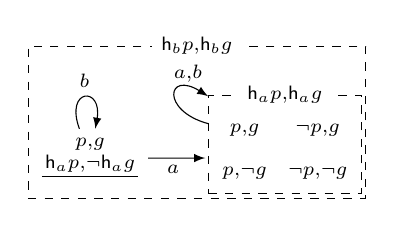
\begin{tikzpicture}\tikzset{deepsquare/.style ={rectangle,draw=black, inner sep=1.5pt, very thin, dashed, minimum height=3pt, minimum width=1pt, text centered}, 
					world/.style={node distance=6pt}, designated/.style={node distance=6pt}
					% world/.style={node distance=6pt,fill=black!5,rounded corners}, designated/.style={node distance=6pt,fill=black!20,rounded corners}
				}
				%% True state:
				\node [designated] (!) {$\underline{\s p,g \atop \mathsf{h}_a p, \neg \mathsf{h}_ag}$};
				%Edge true state:
				\path (!) edge [-latex, looseness=7,in=80,out=110] (!) node [above, xshift=-2pt, yshift=22pt] {$\s b$};
				
				%%% INNER SQUARE
				\node [world, right=of !, xshift=20pt, yshift=10pt] (1) {$\s p,g$};
				\node [world, below=of 1, yshift=2pt](2) {$\s p, \neg g$};
				\node [world, right=of 1](3) {$\s \neg p,g$};
				\node [world, right=of 2, below=of 3, yshift=2](4) {$\s \neg p,\neg g$};
				%Deepsquare
				\node [deepsquare, fit={($(1) +(0,4mm)$)(2)(3)(4)}](square) {};
				%Deepsquare name
				\node[fill=white] (square name 1) at (square.north) {$\s \mathsf{h}_ap, \mathsf{h}_ag$};
				%	\node [world, above=of square, yshift=-7pt] (square name 1) {$\s \mathsf{h}_ap, \mathsf{h}_ag$};
				% Deepsquare Loops
				\path (square) edge [-latex,looseness=4.6,in=148,out=165] (square);
				%Name loop
				\node [node distance=6pt,above=of square, xshift=-35pt, yshift=-5pt] (loop name 1) {$\s a,b$};
				
				%BETWEEN SQUARES
				%Anchor
				\node[left=-8pt of square, xshift=-2pt, yshift=-5pt] (anchor1) {};
				\path (!) edge [-latex] (anchor1) node [above, xshift=30pt, yshift=-9pt] {$\s a$};
				%Edge name
				\node[left=-3pt of square, xshift=2pt, yshift=1.5pt] (anchor1) {};
				
				%%OUTER SQUARE
				\node [deepsquare, fit={(square)(!)(square name 1)($(loop name 1) +(0,3mm)$)}](outsquare) {};
				%Name
				\node [fill=white] (outsquare name) at (outsquare.north) {$\s \mathsf{h}_bp, \mathsf{h}_bg$};
				%	\node [world, left=of outsquare, xshift=9pt] (outsquare name) {$\s \mathsf{h}_bp, \mathsf{h}_bg$};
			\end{tikzpicture}
			
			\caption{The pointed Kripke model $(\mathcal{M},w)$. In the figure, $p$ stands for ``the players in the video pass the ball 15 times'', $g$ for ``a clearly visible gorilla crosses the scene''. %We take $p\wedge g$ to represent everything happening in the video. 
				We use the following conventions. % for representing Kripke models.
				%When representing Kripke models here and throughout the rest of the paper, we use the following conventions. 
				Worlds are represented by sequences of literals true at the world. The model above has 5 worlds, 4 of which are inside the inner dashed box. Designated worlds are underlined. Whenever a world appears inside a dashed box, all the literals in the label of that box are also true in the world---and if the label is underlined, all worlds inside are designated. In this model, $\mathsf{h}_b p$ and $\mathsf{h}_b g$ hold in all worlds, and additionally, $\mathsf{h}_a p$ and $\mathsf{h}_a  g$ hold in the worlds of the inner box. The accessibility relations are represented by labelled arrows. An arrow from (or to) the border of a dashed box means that there is an arrow from (or to) all the events inside the box.  
				%States are represented with (possibly not all) the atomic formulas they satisfy. The designated world is $p,g,\mathsf{h}_ap, \neg\mathsf{h}_ag$. The dashed box represents a set of states that all satisfy the formulas that name the box. The inner box then contains four states that all satisfy $\mathsf{h}_ap, \mathsf{h}_ag$, while the outer box contains five states (the whole domain of the model) that all satisfy $\mathsf{h}_bp, \mathsf{h}_bg$. The $a,b$-loop pointing to the inner box point from all worlds in the box to all such worlds.
			}\label{figure:static}
		\end{figure} 
	\end{example}
	%	In the above example we only demonstrated how the static part of the model works, as the update depends on more specific attention dynamics introduced below.
	\section{Principles for Attention Dynamics}
	In this section, we first present the existing attention model~\cite{bolander2015announcements}. We then propose an alternative representation using our edge principles, introduce a variant, and, finally, generalize to
	%	 and move to a variant of that model which is more appropriate for the types of scenarios that we would like to capture. Last, we generalize the model to 
	%	Then, we build on the resulting model by generalizing it to 
	multiple propositions (capturing that agents can pay attention to subsets of $At$).
	
	\subsection{The Existing Model and our Version of it}
	%	An existing model of attention and our principle-based version of it}
As in
%	In
\cite{bolander2015announcements}, attention is represented as a binary construct where agents can either be paying attention to everything that happens or to nothing.  The language they adopt is as the language above, except for their attention atoms $\mathsf{h}_a$, $a\in Ag$, that are not relativised to propositional formulas. 
% As 
The intended meaning of such atoms is that the agent pays attention to everything, so  they can be expressed in our language by
% , for any $a\in Ag$,
letting $\mathsf{h}_a$, $a\in Ag$, be an abbreviation of the formula $\bigwedge_{p\in At} \mathsf{h}_ap.$
Let $H'=\{\mathsf{h}_a\colon a\in Ag \}$. Then $H'\cup At$ is the set of ``atoms'' on which their language is based. %\footnote{We write atoms in quotation marks, as the $\mathsf{h}_a$ are not really atoms in our case, though we could just as well have introduced them as a separate kind of atoms in our language.} 
%	The model they introduce is a DEL model. 
The static part of their model is a Kripke model, where it is assumed that agents are \emph{attention introspective}, namely for all $w,v\in W, a\in Ag,$ and $p\in At$, if $(w,v)\in R_a$ then $\mathsf{h}_a (p)\in V(w)$ iff $\mathsf{h}_a(p)\in V(v)$.\longv{\footnote{This assumption is phrased differently in \cite{bolander2015announcements}, as there $\mathsf{h}_a$ is a primitive formula and the valuation function maps atomic formulas into sets of worlds, while here it maps worlds into sets of atomic formulas. Note also that we are generally not assuming our Kripke models to satisfy attention introspection, as the false belief of Ann in Example~\ref{ex:static} makes clear.}}
%\tobo{OK, now things already break down technically due to the treatment of $h_a$ as an abbreviation. We can not write $h_a \in V(w)$ when $h_a$ is not an atom. And it's not. So mathematically speaking, it doesn't make sense. Solution? Well, technically, the simplest solution is to say that we add a special propositional atom $q$ and then we use $h_a$ as short for $h_a q$ with the intended meaning that $h_a q$ means to pay attention to everything. Alternatively, and maybe more elegant, we define a language $\mathcal{L}'$ that is at $\mathcal{L}$ except we only have atoms $h_a$ instead of atoms $h_a p$. I think the latter solution is probably the cleanest.} 	 
The dynamics are given by the following event models. % and product updates. 
These event models represent situations in which any formula can be announced, true or false, and attentive agents will come to believe it. 
\begin{definition}[Event Model $\mathcal{E}(\varphi)$, \cite{bolander2015announcements}]\label{def: their action model}
	%		 \tobo{So here we define $\mathcal{E}(\varphi)$, but later we define other event models. Your semantics say that the dynamic modality is defined in terms of $\mathcal{E}(\varphi)$, so formally speaking that must be this one. But I don't think that's what you intend. You want to have different notions of satisfaction dependent on what event model $\mathcal{E}$ you're considering. The normal approach is to have the event model inside the dynamic modality. It's only when it's fixed, like for public announcements, that it's not necessary and it suffices to plug a formula in there. The easiest fix here is to define a general dynamic modality as usual based on an event model, so $[(\mathcal{E},E_d)]\varphi$. Then you can plug in whatever event model you want, e.g. for their model, we would write $[\mathcal{E}(\varphi)] \psi$ and for our first model, we would write $[\mathcal{E}'(\varphi)]\psi$. Or you can solve it another way that you find better. E.g. you might notationally prefer something like $[\varphi]_\mathcal{E} \psi$, I don't know. Just note that the notation $[\mathcal{E}(\varphi)] \psi$ would be the *completely* standard in DEL, and hence everybody familiar with DEL would immediately get it.}
	Given a $\varphi\in \mathcal{L}$, the multi-pointed event model  $\mathcal{E}(\varphi)=((E,Q,pre), E \setminus \{ s_\top\} )$ is defined by: 
	
	$E=\{(i,J)\colon i\in\{0,1\}\text{ and } J\subseteq Ag\}\cup \{s_\top\};$
	
	%		$\mathsf{Q}$ maps each agent $a\in Ag$ to 
	
	\noindent \hspace{1mm}
	\begin{tabular}{ll}
		$Q_a=$&$\{((i,J),(1,K))\colon i\in \{0,1\}, J,K\subseteq Ag \text{ and }a\in J\}\ \cup $\\
		&$\{((i,J),s_\top )\colon i\in \{0,1\}, J\subseteq Ag \text{ and }a\notin J\};$
	\end{tabular}
	
	%		\smallskip
	$pre\colon E\rightarrow \mathcal{L}$ is defined as follows, for $J\subseteq Ag$:
	\vspace{-1mm}
	\begin{itemize}
		\item [-] $pre((0,J))=\neg \varphi\wedge \bigwedge_{a\in J} \mathsf{h}_a \wedge \bigwedge_{a\not\in J} \neg \mathsf{h}_a;$
		\item [-] $pre((1,J))=\varphi\wedge \bigwedge_{a\in J} \mathsf{h}_a \wedge \bigwedge_{a\not\in J} \neg \mathsf{h}_a;$
		\item [-] $pre(s_\top)=\top$. 
	\end{itemize}
	
	%\smallskip
	%$E_d=$.
	%\tobo{I find that formulation a bit odd. You just want to define the multi-pointed version of their model, right? By definition, $(\mathcal{E}(\varphi),E^*_d)$ is a multi-pointed event model, so it's not clear what you want to say here. But I think there is also an issue with how the designated events are dealt with. The semantics define $(\mathcal{M},w)^\varphi = (\mathcal{M},w) \otimes \mathcal{E}(\varphi)$. For this to make sense, $\mathcal{E}(\varphi)$ has to be a multi-pointed event model. Otherwise it doesn't fit the product update definition. And intuitively it's also what we want: If the dynamic modality is defined in terms of $\mathcal{E}(\varphi)$, then $\mathcal{E}(\varphi)$ also need to specify what the designated events are. So either $\mathcal{E}(\varphi)$ should be the event model including the designated events, i.e, $((E^*,Q^*,pre^*),E_d)$, or otherwise the semantics have to be redefined to take both an event model $\mathcal{E}(\varphi)$ and a set of designated events $E_d$. So e.g. instead of writing $(\mathcal{M},w)^\varphi = (\mathcal{M},w) \otimes \mathcal{E}(\varphi)$, it would be something like $(\mathcal{M},w)^\varphi = (\mathcal{M},w) \otimes (\mathcal{E}(\varphi),E_d)$. But in my view, the designated events are part of the model, so I strongly prefer something like the first version, where the event model we refer to is the one that includes a specification of the designated events.} \noteG{Is this issue solved now?}
\end{definition}
This event model contains $2^{|Ag|+1}+1$ events~\cite{bolander2015announcements}. The preconditions of these events express whether the announced $\varphi$ is true (i.e., whether it occurs positively or negatively in the precondition) and whether each agent $a$ is attentive or not (i.e., whether $\mathsf{h}_a$ occurs positively or negatively in the precondition). We now briefly explain the intuition behind the edges of the model, but refer to~\cite{bolander2015announcements} for more details.
The elements of $Q_a$ of the form $((i,J),(1,K))$ encode the following: Provided that agent 
$a$ is attentive (i.e., $a\in J$), she believes that any event with precondition $\varphi$ could be the actual one.
%	, including all events where she is not paying attention (by attention introspection it follows anyway that the states preserved by the update are the ones where the agent knows that she is paying attention).\footnote{We keep the explanation brief and refer to~\cite{bolander2015announcements} for a more detailed description.}  
The elements of $Q_a$ of the form $((i,J),s_\top)$ then encodes:
If instead she is not paying attention (i.e., $a\not\in J$), she keeps the beliefs she had before the announcement (represented by the event $s_\top$ having the precondition $\top$. The $s_\top$ event induces a copy of the original model, thereby modeling the ``skip'' event where nothing happens).

In the following, for any set $S$, we use $id_S$ to denote the identity function on $S$, i.e., $id_S(s) = s$, for all $s \in S$. From now on, most of our event models will be of a particular form where the set of events is a set of (conjunctive) formulas and where preconditions are given by the identify function on $E$, i.e., $pre = id_E$ (meaning that the events are their own preconditions). Our principle-based version of $\mathcal{E}(\varphi)$ is then the following.
\begin{definition}[Principle-Based Event Model $\mathcal{E}'(\varphi)$]\label{a-star-varphi} Given a $\varphi\in \mathcal{L}$, the multi-pointed event model $\mathcal{E}'(\varphi)=((E,Q, id_{E}), E\setminus \{ \top \})$ is: % defined by:
	
	$E=\{\psi \wedge  \bigwedge_{a\in J} \mathsf{h}_a \wedge \bigwedge_{a\not\in J} \neg \mathsf{h}_a\colon \psi\in  \{\varphi,\neg\varphi\}, J\subseteq Ag\}\cup\{\top\};$
	%	\tobo{The similarity of $T$ and $\top$ make the definition hard to parse. I would suggest to call the set $T$ something else.} \tobo{Also, formally speaking, we are not taking elements from $H$, as you defined $h_a$ by abbreviation.}  \noteG{Ok now I used Y, is it ok? Also, I defined $H'$ but I am a bit uncertain about the definition of the set (see above, right under the displayed $\mathsf{h}_a$ formula), and of the notation $H'$.}
	%	\tobo{I have until now assumed that preconditions of events where conjunctions of literals. That means we can then only announce atoms. Maybe it can be generalised, but I'm a bit afraid of doing that right now. And when we end up presented *our* model, event preconditions *will* be conjunctions of atoms. So for now I assume that we will eventually restrict their model to announcing atoms, and just put a note that it can be generalised.}
	% \tobo{Here mathsf is used for event models, but so far they were mathcal. I would suggest to use the same font for all event models.} 
	%	
	
	%		\smallskip
	$Q_a$ is such that $(e,f)\in Q_a$ iff all the following are true:
	\vspace{-1mm}
	\begin{itemize}
		\item[-] \textsc{Basic Attentiveness}: if $\mathsf{h}_a\in e,$ then $\varphi\in f$;
		
		\item[-] \textsc{Inertia}: if $\mathsf{h}_a \not\in e$, then $f = \top$.
		%		 
		%		 \item[-] Top: if $e=\top$ then $f=\top$
	\end{itemize} 
	%	 \noteG{About Top: we could either bundle it with Inertia, or called it something like \emph{null} or something that points out that nothing happens there. Like in July or Tuesdays, they say...} \tobo{I think I might prefer to formulate it as ``if $e = \top$ then $f = \top$''. And for inertia, ``if $\neg h_a \in e$ then $f = \top$''. Concerning the name of the last principle, can't we combine inertia and top to one principle? This would be: ``if $h_a \not\in e$, then $f = \top$''. Why would that work? Call my new principle Inertia$^*$. Then I prove that Inertia + Top is equivalent to Inertia$^*$. Left to right: Assume Inertia + Top. Suppose $h_a \not\in e$. We need to prove $f = \top$. Since $h_a \not\in e$, either $\neg h_a \in e$ or $e = \top$. If $\neg h_a \in a$, by inertia $f = \top$. If $e = \top$, then by Top, $e = f = \top$. This proves left to right. Right to left: Suppose Inertia$^*$. We first prove inertia. To do this, suppose $\neg h_a \in e$. Then we need to prove $f = \top$. From $\neg h_a \in e$ we  get $h_a \not\in e$, by definition of the events of our event model. Inertia$^*$ then gives $f= \top$, as required. Now we prove Top. To do this, suppose $e = \top$. Then again $h_a \not\in e$, and by Inertia$^*$ we get $f = \top$. This concludes the proof. So we don't need to invent new names, we can simply reduce everything to attentiveness and inertia if we just generalise inertia a bit.}\noteG{Amazing!}
	
	
	%	$pre(e)=e$ 
	%	\tobo{Here we can consider to do as I do later and simple plug in $id_E$ as the third element of the tuple already in the beginning, so that we don't need a separate clause for $pre$. So in the beginning of Def 6, write ``the action model $A_\varphi^* = (E^*,Q*,id_{pre})$ is defined by''. This requires us to first write a comment about identity functions and using the identity as the precondition function, but there's already a bit about this in the first paragraph of the section, it just has to be revised a bit.} 
	%		 
	
	%\noindent \hspace{0mm}
	%\smallskip
	%$E_d=$. % is the set of designated events.
\end{definition}


The \emph{edge principles} of the model above are \textsc{Basic Attentiveness} and \textsc{Inertia}%	. These describe 
, describing the conditions under which there is an edge from $e$ to $f$ for agent $a$, that is, what an agent considers possible after the announcement.
By \textsc{Basic Attentiveness}, paying attention implies that, in all events considered possible, the announcement is true---and hence attentive agents believe what is announced. By \textsc{Inertia}, inattentive agents believe nothing happened, namely they maintain the beliefs they had before the announcement was made. 

Note that we have exactly the same set of event preconditions in $\mathcal{E}'(\varphi)$ as in $\mathcal{E}(\varphi)$. The difference is just that we define the events to be their own preconditions, which is possible since all pairs of events have distinct and mutually inconsistent preconditions. It's easy to check that $\mathcal{E}(\varphi)$ and $\mathcal{E}'(\varphi)$ also have the same edges, hence the models are isomorphic. The following proposition shows this.
%(we prove this in the Supplementary Material).

\begin{proposition}
	$\mathcal{E}(\varphi)$ of Definition 3.1 and  $\mathcal{E}'(\varphi)$ of Definition 3.2 are isomorphic.
\end{proposition}
\begin{proof} %[Proof that ]
	We already concluded that the two models have the same set of preconditions, and that all events have distinct preconditions. We then just need to show that for all $a \in Ag$ and all events $e,f \in E$ of $\mathcal{E}(\varphi)$, we have $(e,f) \in Q_a$ in $\mathcal{E}(\varphi)$ iff $(pre(e),pre(f)) \in Q_a$ in $\mathcal{E}'(\varphi)$. To see this, consider first an edge in $Q_a$ of $\mathcal{E}(\varphi)$. It's either of the form $((i,J),(1,K))$ for some $i\in \{0,1\}, J,K\subseteq Ag$ and $a\in J$ or it's of the form $((i,J),s_\top)$ for some $i\in \{0,1\}, J\subseteq Ag$ and $a \not\in J$. According to Definition~3.1, an edge of the first form is an edge from an event with precondition $\neg \varphi\wedge \bigwedge_{a\in J} \mathsf{h}_a \wedge \bigwedge_{a\not\in J} \neg \mathsf{h}_a$ or $\varphi\wedge \bigwedge_{a\in J} \mathsf{h}_a \wedge \bigwedge_{a\not\in J} \neg \mathsf{h}_a$  to an event with precondition $\varphi\wedge \bigwedge_{a\in K} \mathsf{h}_a \wedge \bigwedge_{a\not\in K} \neg \mathsf{h}_a$. Such an edge clearly satisfies \textsc{Basic Attentiveness} (since $\varphi$ is a conjunct of the target of the edge) and \textsc{Inertia} (the condition $a \in J$ for the source event implies that $\mathsf{h}_a$ is contained in the precondition of the source, and hence \textsc{Inertia} holds trivially). This shows that edges in $\mathcal{E}(\varphi)$ of the first type are also edges in $\mathcal{E}'(\varphi)$. The argument for edges of the second type is similar, but here the condition of the source is $a \not\in J$, meaning that \textsc{Basic Attentiveness} instead is trivial, and we only need to show \textsc{Inertia}. According to Definition~3.1, an edge of the second type is an edge from an event with precondition $\neg \varphi\wedge \bigwedge_{a\in J} \mathsf{h}_a \wedge \bigwedge_{a\not\in J} \neg \mathsf{h}_a$ or $\varphi\wedge \bigwedge_{a\in J} \mathsf{h}_a \wedge \bigwedge_{a\not\in J} \neg \mathsf{h}_a$ (as before) to an event with precondition $\top$. Since $a \not\in J$, we have that $\mathsf{h}_a$ is not contained in the precondition of the source event. \textsc{Inertia} then requires that the precondition of the target is $\top$, but that we already concluded. So \textsc{Inertia} holds, as required.
	
	For the other direction, we start with an edge $(e,f) \in Q_a$ of $\mathcal{E}'(\varphi)$ satisfying both \textsc{Basic Attentiveness} and \textsc{Inertia}, and show that it is of one of the two types in $\mathcal{E}(\varphi)$. We split into cases depending on whether $\mathsf{h}_a \in e$ or not. If $\mathsf{h}_a \in e$, then by \textsc{Basic Attentiveness}, $\varphi \in f$. Let $J$ denote the set of agents for which $\mathsf{h}_a$ occurs positively in $e$, and let $K$ denote the same set for $f$. Since  $\mathsf{h}_a \in e$, we get $a \in J$. Let $i=0$ if $\neg \varphi$ occurs in $e$, otherwise let $i=1$. Then $e = pre((i,J))$, using the notation from Definition~3.1. Since $\varphi \in f$, we have that $f = pre((1,K))$. By Definition~3.1, $Q_a$ contains an edge from $(i,J)$ to $(1,K)$. This covers the case where $\mathsf{h}_a \in e$. Consider now the case $\mathsf{h}_a \not\in e$. By \textsc{Inertia}, $f = \top$. Define $J$ and $i$ as before from $e$. Then, as before, $e = pre((i,J))$. Since $f = \top$, $f = pre(s_\top)$. By Definition~3.1, $Q_a$ contains an edge from $(i,J)$ to $s_\top$, and we're done.  
\end{proof}


%The set of events is now a set of conjunctive formulas, that specify whether $\varphi$ or $\neg \varphi$ is the case and whether $\mathsf{h}_a$ or $\neg \mathsf{h}_a$, for all $a\in Ag$ is the case (hence, we still have $2^{n+1}+1$ events, where $n$ is the number of agents). This matches the assumption that announcements may be false, and that any combination of attention attitudes may be considered possible. 
%	What an agent considers possible after the announcement is now clearly and explicitly captured by the principles. By \textsc{Basic Attentiveness}, paying attention implies that, in all events considered possible, the announcement is true---and hence attentive agents believe what is announced. By \textsc{Inertia}, inattentive agents believe nothing happened, namely they maintain the beliefs they had before the announcement was made. % \noteG{[the following parenthesis is now a repetition too, I think]}($\top$ is the ``skip'' event representing that nothing happens).
%	by definition of $E$, if $\mathsf{h}_a\notin e$ then $\mathsf{h}_a\notin J$, and so $\neg \mathsf{h}_a \in e$. Hence Inertia implies that if $\neg \mathsf{h}_a \in e$ then $f = \top$, where $\top$ is the ``skip'' event where nothing happens).


Compare the edge specification from $\mathcal{E}(\varphi)$ with the one from $\mathcal{E}'(\varphi)$. We are defining the same set of edges, but whereas the definition of $Q_a$ in $\mathcal{E}(\varphi)$ does not make it immediately clear what those edges are encoding, we believe that our definition of $Q_a$ in $\mathcal{E}'(\varphi)$ does. It is simply two basic principles, one specifying what events are considered possible by the agents paying attention (\textsc{Basic Attentiveness}), and another specifying the same for those not paying attention 
%	what events are considered possible by agents not paying attention 
(\textsc{Inertia}). 
%We call it Inertia, since it's a principle of epistemic inertia:  If nothing has been seen or heard to have changed, it's believed that nothing changed.
%	\noteG{[I think we do not need the following sentence, as we explained above what inertia means:]}\noteG{The latter is indeed a principle of epistemic inertia: If the agent doesn't see anything changed, she believes nothing has changed.} % \noteG{Hidden below here there is some text that I think is a bit repetitive, as it seems to me that we already explained how to read the principles. Also, I took the skippy thing and moved it above.}
%[The way to read the Attentiveness principle is: If an agent pays attention in $e$ and considers another event $f$ possible, then $\varphi$ must be contained in that event ($\varphi$ ``happens'' in that event). The Intertia principle can be read as: If an agent doesn't pay attention in $e$ and considers another event $f$ possible, then that other event must be $\top$ (the ``skip'' event where nothing happens).] 
Even though from a technical viewpoint it is not a big step to introduce such principles, we find it helpful to be able to specify the relevant event models in a clear and concise manner. %, mainly as the model is then more transparent, in the sense that it is clearer what moving parts there are and what their function is. 
This makes it easier to use the model and build on it---as should become evident when we later generalise the event model. % to handle propositional attention and defaults. 
\subsubsection{Modified model} 
We now introduce a variant of the event model
$\mathcal{E}'(\varphi)$ from %of 
Def. \ref{a-star-varphi}, 
one that is more appropriate for the types of scenarios that we would like to be able to model. 
%	We now introduce a variant of the event model $\mathcal{E}'(\varphi)$ of Def. \ref{a-star-varphi}, that gives up some of the assumptions underlying it. \noteG{Here i moved your formulation to the beginning of the section, as I thought that it was fitting there. But now this part looks less elegant, so I don't know if you will like it.}
\paragraph{Truthful announcements} As the present work aims at modeling (noise-free) attention to external stimuli from the environment, in particular visual attention, the first assumption we give up is that announcements may be false. %\noteG{[Here we had three ways to say the same. I reduced it to two. Maybe we can reduce to one?]}Our events are always truthful: nature reveals itself to the attentive agents. 
More precisely, we assume that 
%	if an agent pays attention to something, and if that something is revealed, then the agent sees it the way it truly is (later we will make this more precise and say that 
if an agent pays attention to $p$ and the truth-value of $p$ is being revealed, then the agent sees the true truth-value of $p$.
%).   
%	$p$ and the truth-value of $p$ is being revealed, then the agent sees the true truth value of $p$. %\noteG{@Thomas: see how new age this is, then I ll change it as it doesn't fit.} 
The new event model for announcing $\varphi$ should then only contain events where $\varphi$ is true:
%		\begin{definition}[Truthful Event Model $\mathcal{A}'_\varphi$]
	%		Given a formula $\varphi\in \mathcal{L}$, the action model $\mathcal{A}'_\varphi=(E', {Q}', id_{E'})$, where ${Q}', id_{pre}$ are as in Def. \ref{def: their action model}, and ${E}'$ is given by:
	%		
	%	\end{definition}	

\begin{center}
	$E=\{\varphi \wedge  \bigwedge_{a\in J} \mathsf{h}_a \wedge \bigwedge_{\mathsf{h}_a\not\in J} \neg \mathsf{h}_a\colon  J\subseteq Ag\}\cup\{\top\}.$
\end{center}
\paragraph{Learning that you were attentive}
An assumption we have already given up is attention introspection, so in our models the agents may falsely believe to be paying attention (see Example \ref{ex:static}). 
%%	While attention introspection is a property of static Kripke models, in situations of false beliefs about the agents' own attention, if they are actually paying attention and thus learn what the true event is, it is plausible to assume that they also learn that they were attentive.
%\noteG{
	In this setting, 
	%Although attention introspection is a property of static Kripke models,
	it is very plausible to assume that, besides learning what the true event is, attentive agents also learn that they were attentive.
	%}
This does not happen in the event model $\mathcal{E}'(\varphi)$. We thus substitute \textsc{Basic Attentiveness} with the following principle:
\begin{itemize}
	\item [-] \textsc{Attentiveness}: if $\mathsf{h}_a\in e,$ then $\mathsf{h}_a,\varphi \in f$.
\end{itemize}
Summing up, the event model where announcements are truthful and attentive agents learn that they paid attention, looks as follows.
\begin{definition}[Truthful and Introspective Event Model $\mathcal{E}''(\varphi)$] \label{truthful and introspective}
	Given $\varphi\in \mathcal{L}$, the multi-pointed event model $\mathcal{E}''(\varphi)=((E, Q, id_{E}), E\setminus \{ \top \})$ is defined by:
	
	$E=\{\varphi \wedge  \bigwedge_{a\in J} \mathsf{h}_a \wedge \bigwedge_{a\not \in J} \neg \mathsf{h}_a\colon  J\subseteq Ag\}\cup\{\top\}$;
	
	\smallskip
	$Q_a$ is such that $(e,f)\in Q_a$ iff all the following are true:
	\begin{itemize}
		\item[-] \textsc{Attentiveness}: if $\mathsf{h}_a\in e,$ then $\mathsf{h}_a,\varphi \in f$;
		\item[-] \textsc{Inertia}: if $\mathsf{h}_a \not\in e$, then $f = \top$;
	\end{itemize} 
	
	%\smallskip
	%		$E_d=$. % is the set of designated events.
\end{definition}	
The event model 
$\mathcal{E}''(p \land g)$ with $Ag = \{a,b\}$  is shown in Figure~\ref{fig: event introspective}. %It is the event model for truthfully announcing $p \land g$ to agents that may pay attention or not. 
\begin{figure}
	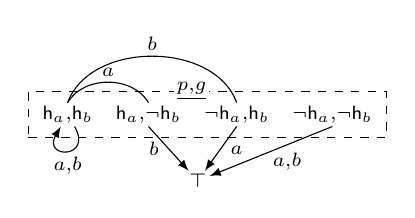
\begin{tikzpicture}\tikzset{deepsquare/.style ={rectangle,draw=black, inner sep=1pt, thin, dashed, minimum height=3pt, minimum width=1pt, text centered}, 
			world/.style={node distance=6pt,inner sep=1pt},auto}
		
		%% True state:
		\node [world] (1) {${\s \mathsf{h}_a,  \mathsf{h}_b}$};
		\node [world, right=of 1] (2) {${\s \mathsf{h}_a, \neg \mathsf{h}_b}$};
		\node [world, right=of 2] (3) {${\s \neg \mathsf{h}_a, \mathsf{h}_b}$};
		\node [world, right=of 3] (4) {${\s \neg \mathsf{h}_a,  \neg \mathsf{h}_b}$};
		\node [world, below=of 1, xshift=47pt, yshift=-10pt] (5) {$\s \top$};
		
		%Edges:
		\path (1) edge [-latex,loop,looseness=7,in=240,out=300] node[yshift=0.5mm] {$\s a,b$}  (1);
		
		%	\node[left=-16pt of 2, yshift=-2pt] (anchor1) {};
		\path (2.south) edge [-latex]  node[left] {$\s b$} (5);
		
		%	\node[left=-23pt of 3, yshift=-3pt] (anchor2) {};
		\path (3.south) edge [-latex]  node[yshift=1.5mm]  {$\s a$} (5);
		
		%	\node[left=-23pt of 4, yshift=-4pt] (anchor3) {};
		
		\path (4.south) edge [-latex] node[xshift=-1mm,yshift=1mm]  {$\s a,b$} (5);
		
		%				\node[above=-5pt of 1] (anchor4) {};
		%				\node[above=-5pt of 2] (anchor5) {};
		%				\node[above=-5pt of 3] (anchor6) {};
		%		\path[-] (1) edge[bend left=60] (2) node [below, xshift=15pt, yshift=13.5pt] {$\s a$};
		\path[-] (1.north) edge[bend left=60] node[yshift=-0.5mm] {$\s a$} (2.north);		
		
		%		\path[-] (1) edge[bend left=60] (3) node [below, xshift=35pt, yshift=20pt] {$\s b$};
		\path[-] (1.north) edge[bend left=70] node[yshift=-0.5mm] {$\s b$} (3.north) ;
		
		%Square:
		\node[deepsquare, inner sep=4pt, fit={(1)(2)(3)(4)}] (announcement) {};
		\node[fill=white,inner sep=1pt,xshift=-2mm] (square name 1) at (announcement.north) {\underline{$\s p, g$}};
		%	\node[left=0pt of 1, yshift=-1pt] (anchor2) {$\s p\wedge g$};
	\end{tikzpicture}
	\caption{The event model $\mathcal{E}''(p\wedge g)$ with $Ag = \{a,b\}$. As our event models will have conjunctive preconditions, all distinct, and our events are their own preconditions, we can represent events by lists of formulas, the formulas contained in the event precondition. 
		All other conventions are as for Kripke models (see Fig.~\ref{figure:static}).	
		% with one addition:
		%		 We use the same conventions as for Kripke models, with one additional convention: 
		%if the label of a dashed box is underlined, then all the events inside it are designated. In this event model, the leftmost event is designated and has precondition $\mathsf{h}_a \land \mathsf{h}_b \land p \land g$. % (where the two last conjuncts come from the dashed box).
		%Events are represented by their name, which is also their precondition. The convention is that all events $e$ in the dashed box have the formula that names the box as part of their precondition (in this case $p\wedge g$, so $p\wedge g\in e$). All events are designated except the null event $\top$. 
		%	 The edges satisfy Introspective Attentiveness and Inertia. %, and double arrows are indicated with undirected edges.
	}
	\label{fig: event introspective}
\end{figure}
\subsection{Event Models for Propositional Attention}

In this section, we introduce event models for agents that only pay attention to  subsets of $At$.  
%pay attention only to a part of the event model, and thus learn only partially what happens. 
As our main aim  is to model attention to external stimuli, we are interested in modeling the ``announcement'' of a conjunction of literals $(\neg) p_1 \wedge \dots \wedge (\neg) p_n$, which we interpret as the parallel exposure to multiple stimuli (the truth value of all $p_i$ being revealed concurrently). It could for instance be that we see a video that has 15 ball passes and a gorilla passing by, and that would correspond to the ``announcement'' $p \land g$, cf.\ Example	~\ref{ex:static}. 
\begin{definition}[Propositional Attention Event Model $\mathcal{F}(\varphi)$]\label{e-varphi} Let $\varphi=\ell(p_1)\wedge \dots \wedge \ell(p_n) \in \mathcal{L}$, where for each $p_i$, either $\ell(p_i)=p_i$ or $\ell(p_i)=\neg p_i$. 
	%	 each $\ell(p_i)$ is a literal containing the propositional atom $p_i$ (so $\ell(p_i) = p_i$ or $\ell(p_i) = \neg p_i$). 
	The multi-pointed event model $\mathcal{F}(\varphi)=((E,Q,id_{E}), E_d)$ is defined by:
	%		
	%		$$E=\{\bigwedge S \wedge  \bigwedge_{a \in Ag \atop \ell(p_i) \in X_a} \mathsf{h}_a p_i \wedge \bigwedge_{
		%		a \in Ag \atop \ell(p_i) \in S \setminus X_a} \neg \mathsf{h}_a p_i  \colon$$ 
	%		$$S \subseteq \mathit{Lit}(\varphi) \text{ and for all $a \in Ag$, $X_a \subseteq S$} \}$$
	\begin{multline*}
		%	E=\{\bigwedge S \wedge  \bigwedge_{a \in Ag \atop \ell(p_i) \in X_a} \mathsf{h}_a p_i \wedge \bigwedge_{
			%		a \in Ag \atop \ell(p_i) \in S \setminus X_a} \neg \mathsf{h}_a p_i  \colon \\S \subseteq \mathit{Lit}(\varphi) \text{ and for all } a \in Ag,X_a \subseteq S \}
		%\end{multline*}
		%\tobo{Or, alternatively e.g.: 
			%\begin{multline*}
			E=\{\bigwedge_{p \in S} \ell(p) \wedge  \bigwedge_{a \in Ag} \bigl(\bigwedge_{p \in X_a} \mathsf{h}_a p \wedge \bigwedge_{p \in S \setminus X_a} \neg \mathsf{h}_a p \bigr)  \colon \\S \subseteq \mathit{At}(\varphi) \text{ and for all } a \in Ag,X_a \subseteq S \}
		\end{multline*}
		%If we make this change, probably it would also be best to replace $p_i$ by $p$ everywhere below. 
		%}		
	\smallskip
	$Q_a$ is such that $(e,f)\in Q_a$ iff all the following hold for all $p$: % \in At(\varphi)$:
	
	\vspace{-1mm}
	\begin{itemize}
		\item[-] \textsc{Attentiveness}: if $\mathsf{h}_a p\in e$ then $\mathsf{h}_a p, \ell(p)\in f$;
		\item[-] \textsc{Inertia}: if $\mathsf{h}_a p\notin e$ then $\ell(p)\not\in f;$
	\end{itemize}  %\noteG{hidden below the principles in their old form.}
	
	%
	%
	%\noteG{the principles above are a shortened version, so to match what we have above. These are the original principles that we had on the whiteboard:
		%	\begin{itemize}
			%\item[-] Attentiveness 1: if $\mathsf{h}_ap\in e$ then $\ell(p)\in f$;
			%\item[-] Attentiveness 2: if $\mathsf{h}_ap\in e$ then $\mathsf{h}_ap\in f$;
			%\item[-] Inertia 1: if $\neg \mathsf{h}_ap\in e$ then $\ell(p)\not\in f;$
			%\item[-] Inertia 2: if $\ell(p)\notin e$ then $\ell(p)\notin f$;
			%\end{itemize} }
			%\noindent $id_E$ is the identity function on $E$;\\
			$E_d=\{\psi\in E\colon \ell(p)\in \psi, \text{ for all } \ell(p)\in \varphi\}$. % is the set of designated events.
		\end{definition}
		
		In  $\mathcal{F}(\varphi)$ we have, for each subset of literals in $\varphi$, an event containing those literals in the precondition. For those literals, the event also specifies whether each agent is paying attention to it or not. In this way, events account for all possible configurations of attention to any subset of the announcement and for the learning of truthful information regarding it. The edges are again given by two simple principles. %, which have similar meaning to the principles introduced above. 
		\textsc{Attentiveness} states that if an agent pays attention to a specific atom, then she learns the literal in the announcement corresponding to it and that she was paying attention to it. \textsc{Inertia} says that if an agent doesn't pay attention to an atom, then she will not learn anything about it. As we take announcements as truthful revelations, the set of designated events only contains events where all the announced literals are true.
		%(we then call them ``maximal events'')
		The event model $\mathcal{F}(\varphi)$ with $\varphi = p \land g$ and $Ag = \{a,b\}$ is shown in Figure~\ref{figure:monster}.
		
		%		All the maximal events are designated, so this is a multi-designated event model. We understand $\top$ as the event where nothing happened.
		
		%		\textbf{Remark}. Note that we have one event per boolean combination of the atoms $\mathsf{h}_ap$, $a \in Ag$. 
		%		
		%\tobo{I'm deleting some comments and remarks that seem obsolete by now. They have been covered earlier. And if some of them haven't been sufficiently covered earlier, they *should* have. If we want to something about the meaning of $\top$, say, then of course we should say it the very first time we use $\top$ as an event precondition.} 
		
		
		%		Note that because of Introspective Attentiveness, agents learn that they are paying attention. In propositional attention settings, this is necessary: if an agent did not learn that she paid attention, then she might consider it possible that she is not paying attention and so by Inertia also that nothing happened. This would be against the idea that when agents are paying attention they gain a new belief in the truth of the announcement. \tobo{If you want this argument to be in here, I think you need to elaborate it technically. There seem to be something about transitivity going on here? It would be nice if you indeed connected it to the formal definition, it would also add to the technical meat of the paper. Without transitivity, I'm not sure your point holds?} \noteG{Indeed, I think it doesn't. I will remove it when I work on this paragraph (tomorrow, if I manage with the picture)} \tobo{Yes, so maybe that part should just go out, it'll save us both time and space.}
		\begin{figure}
		\begin{center}
		\includegraphics[width=0.5\textwidth]{monstermodel}
			\caption{The event model $\mathcal{F}(p\wedge g)$ with $Ag = \{a,b\}$. Solid arrows are for agent $a$, dotted for agent $b$. %Convention for dashed boxes and designated events are the same as above.
			}	\label{figure:monster}
			\end{center}
		\end{figure}
		
		\begin{example} 
			Continuing Example \ref{ex:static}, Ann and Bob have finished watching the Invisible Gorilla video (event model $\mathcal{F}(p\wedge g)$). As Bob expected, Ann learns that there are 15 ball passes, %players pass the ball 15 times, 
			but she still doesn't know anything about whether there is a gorilla in the video, and believes Bob is in the same situation as herself. % her same situation.
			The pointed Kripke model $(\mathcal{M}',w') = 
			(\mathcal{M},w)\otimes\mathcal{F}(p\wedge g)$ in Figure \ref{figure:update} (left) represents the situation after exposure to the video, i.e., after the revelation of $p\wedge g$.  Ann has only learnt about $p$ and 
			%				is still uncertain about $g$. 
			still has no information about $g$. We thus have $(\mathcal{M}',w') \vDash B_a p\wedge \neg B_a g \land \neg B_a \neg g$. Moreover, she wrongly believes Bob too hasn't received any information about the gorilla, so $(\mathcal{M}',w') \vDash B_b g \land B_a(\neg B_b g \land \neg B_b \neg g)$. % Bob instead has correctly learnt that Ann didn't learn about the gorilla, i.e., $(\mathcal{M}',w') \vDash B_b (\neg B_a g \land \neg B_a \neg g)$.
			
			\begin{figure}
				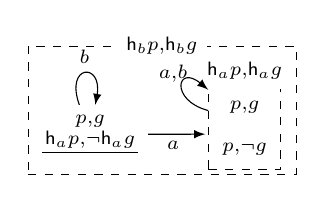
\begin{tikzpicture}\tikzset{deepsquare/.style ={rectangle,draw=black, inner sep=1.5pt, very thin, dashed, minimum height=3pt, minimum width=1pt, text centered}, 
						world/.style={node distance=6pt}, designated/.style={node distance=6pt}
						% world/.style={node distance=6pt,fill=black!5,rounded corners}, designated/.style={node distance=6pt,fill=black!20,rounded corners}
					}
					%% True state:
					\node [designated] (!) {$\underline{\s p,g \atop \mathsf{h}_a p, \neg \mathsf{h}_ag}$};
					%Edge true state:
					\path (!) edge [-latex, looseness=7,in=80,out=110] (!) node [above, xshift=-2pt, yshift=22pt] {$\s b$};
					
					%%% INNER SQUARE
					\node [world, right=of !, xshift=20pt, yshift=10pt] (1) {$\s p,g$};
					\node [world, below=of 1, yshift=2pt](2) {$\s p, \neg g$};
					%Deepsquare
					\node [deepsquare, fit={($(1) +(0,4mm)$)(2)}](square) {};
					%Deepsquare name
					\node[fill=white] (square name 1) at (square.north) {$\s \mathsf{h}_ap, \mathsf{h}_ag$};
					% Deepsquare Loops
					\path (square) edge [-latex,looseness=5,in=140,out=165] (square);
					%Name loop
					\node [node distance=6pt, xshift=30pt, yshift=22pt] (loop name 1) {$\s a,b$};
					
					%BETWEEN SQUARES
					%Anchor
					\node[left=-8pt of square, xshift=-2pt, yshift=-5pt] (anchor1) {};
					\path (!) edge [-latex] (anchor1) node [above, xshift=30pt, yshift=-9pt] {$\s a$};
					%Edge name
					\node[left=-3pt of square, xshift=2pt, yshift=1.5pt] (anchor1) {};
					
					%%OUTER SQUARE
					\node [deepsquare, fit={(square)(!)(square name 1)($(loop name 1) +(0,3mm)$)}](outsquare) {};
					%Name
					\node [fill=white] (outsquare name) at (outsquare.north) {$\s \mathsf{h}_bp, \mathsf{h}_bg$};
					%	\node [world, left=of outsquare, xshift=9pt] (outsquare name) {$\s \mathsf{h}_bp, \mathsf{h}_bg$};
				\end{tikzpicture} \qquad \quad
				\begin{tikzpicture}\tikzset{deepsquare/.style ={rectangle,draw=black, inner sep=1.5pt, very thin, dashed, minimum height=3pt, minimum width=1pt, text centered}, 
						world/.style={node distance=6pt}, designated/.style={node distance=6pt}
						% world/.style={node distance=6pt,fill=black!5,rounded corners}, designated/.style={node distance=6pt,fill=black!20,rounded corners}
					}
					%% True state:
					\node [designated] (!) {$\underline{\s p,g \atop \mathsf{h}_a p, \neg \mathsf{h}_ag}$};
					%Edge true state:
					\path (!) edge [-latex, looseness=7,in=80,out=110] (!) node [above, xshift=-2pt, yshift=22pt] {$\s b$};
					
					
					%%% BELIEVED WORLD
					\node [world, right=of !, xshift=15pt, yshift=0.5pt] (1) {$\s p, \neg g, \atop  \mathsf{h}_a p,\mathsf{h}_a g$};
					% a,b-BELIEVED STATE LOOP
					\path (1) edge [-latex, looseness=7,in=80,out=110]  node [above] {$\s a,b$} (1);
					
					
					%%% INNER SQUARE
					%						\node [world, right=of !, xshift=20pt, yshift=10pt] (1) {$\s p,g$};
					%						\node [world, below=of 1, yshift=2pt](2) {$\s p, \neg g$};
					%Deepsquare
					%						\node [deepsquare, fit={($(1) +(0,4mm)$)(2)}](square) {};
					%Deepsquare name
					%						\node[fill=white] (square name 1) at (square.north) {$\s \mathsf{h}_ap, \mathsf{h}_ag$};
					% Deepsquare Loops
					%						\path (square) edge [-latex,looseness=5,in=140,out=165] (square);
					%Name loop
					%						\node [node distance=6pt, xshift=30pt, yshift=22pt] (loop name 1) {$\s a,b$};
					
					%BETWEEN SQUARES
					%Anchor
					\node[left=-8pt of square, xshift=-2pt, yshift=-5pt] (anchor1) {};
					\path (!) edge [-latex] (anchor1) node [above, xshift=30pt, yshift=-9pt] {$\s a$};
					%Edge name
					\node[left=-3pt of square, xshift=2pt, yshift=1.5pt] (anchor1) {};
					
					%%OUTER SQUARE
					\node [deepsquare, fit={(square)(!)(square name 1)($(loop name 1) +(1.5,3mm)$)}](outsquare) {};
					%Name
					\node [fill=white] (outsquare name) at (outsquare.north) {$\s \mathsf{h}_bp, \mathsf{h}_bg$};
					%	\node [world, left=of outsquare, xshift=9pt] (outsquare name) {$\s \mathsf{h}_bp, \mathsf{h}_bg$};
				\end{tikzpicture}
				
				
				
				\caption{Pointed Kripke models $(\mathcal{M}',w') = (\mathcal{M},w)\otimes\mathcal{F}(p\wedge g)$ (left) and 
					$(\mathcal{M}'',w'') = (\mathcal{M},w)\otimes\mathcal{E}(p\wedge g, d)$ (right), where the default map $d$ is $d_a(p)=d_b(p)=\top$ and $d_a(g)=d_b(g)=\neg g$.} \label{figure:update}
			\end{figure} 
		\end{example}
		
		%	\begin{proposition} If $M$ satisfies transitivity, euclideannes then $M\otimes\mathcal{E}_p(\varphi)$ does too.\noteG{TODO}
			%		\end{proposition}
		%		\begin{proof}
			%			Obvious :-)
			%		\end{proof}
		%		
		%		\opt{Give an example. For instance, initial model with actual world $h_p$ and another indistinguishable $\neg h_p$ world. The agent doesn't know whether she is paying attention to $p$ or not. After getting exposed to $p$ (or $\neg p$), she will both know $p$ ($\neg p$) and know that she \emph{is} paying attention. E.g. a robot not knowing whether it's touch sensor is functional.} 
		%		
		\section{Axiomatization} %: Logic for Propositional Attention}
	We move to the axiomatization of our logic and show that it is sound and complete. The axiomatization is given by the set of axioms and inference rule of Table \ref{tab:logic}. It comprises standard axioms and inference rules for normal modal logic as well as reduction axioms. All propositional reduction axioms in Table \ref{tab:logic} are for  state-eliminating updates, in that they are relativized to the announced $\varphi$. Then, the only non-standard axiom we introduce is the one expressing the consequences of attention-dependent announcements for what concerns agents' beliefs. Where $\varphi=\ell(p_1)\wedge\dots\wedge \ell(p_n)$ is the announced formula, the axiom is the following:
	\begin{multline*}
		[\mathcal{F}(\varphi)]B_a\psi \leftrightarrow (\varphi \rightarrow \bigvee_{S\subseteq At(\varphi)}\bigl( \bigwedge_{p\in S}\mathsf{h}_ap \wedge \bigwedge_{p\in At(\varphi)\setminus S}\neg \mathsf{h}_ap)\\\rightarrow B_a([\mathcal{F}(\bigwedge_{p\in S} \ell(p)) ]\psi))\bigr)
	\end{multline*}
	The axiom can be read as saying that after exposure to the revelation of $\varphi$,
	%-announcement, 
	agent $a$ believes that only the conjunction of literals from $\varphi$ to which she was paying attention to has been revealed. 
	\begin{table} %[h]
		\caption{\label{tab:logic}The logic of propositional attention $\Lambda$. It is assumed that $\varphi = \ell(p_1)\wedge \dots \wedge \ell(p_n)$ for some literals $\ell(p_i)$, $i = 1,\dots,n$.}
		\begin{tabular}{l}\toprule
			All propositional tautologies\\
			$B_{a}(\varphi\rightarrow \psi)\rightarrow (B_{a}\varphi\rightarrow B_a\psi)$ \\
			%				$B_{a}\varphi\rightarrow B_{a}B_{a}\varphi$ \\
			%				$\neg B_{a}\varphi\rightarrow B_{a}\neg B_{a}\varphi$\\
			$[\mathcal{F}(\varphi)] p \leftrightarrow (\varphi\rightarrow p)$ \\
			$[\mathcal{F}(\varphi)] \neg \psi \leftrightarrow( \varphi \rightarrow \neg [\mathcal{F}(\varphi)]\psi)$ \\
			$[\mathcal{F}(\varphi)](\psi\wedge\chi)\leftrightarrow([\mathcal{F}(\varphi)]\psi\wedge[\mathcal{F}(\varphi)]\chi)$\\
			$[\mathcal{F}(\varphi)]B_a\psi \leftrightarrow (\varphi \rightarrow \bigvee_{S\subseteq At(\varphi)}(( \bigwedge_{p\in S} \mathsf{h}_ap \wedge \bigwedge_{p\in At(\varphi)\setminus S}\neg \mathsf{h}_ap)$ \\ \hfill$\rightarrow B_a([\mathcal{F}(\bigwedge_{p\in S} \ell(p)) ]\psi)))$\\
			From $\varphi$ and $\varphi\rightarrow\psi$, infer $\psi$ \\
			From $\varphi$ infer $B_a\varphi$\\
			From $\varphi\leftrightarrow \psi$, infer $\chi[\varphi\slash p]\leftrightarrow \chi[\psi\slash p]$\footnote{This is standard notation for substitution, although it looks similar to the notation for the dynamic modality.}\\
			\bottomrule
		\end{tabular}
	\end{table}

To prove soundness and completeness of the axiomatization in Table~\ref{tab:logic}, we will use the following lemma, which shows that updating a Kripke model $(\mathcal{M},w)$ with event model $\mathcal{F}(\varphi)$ where $\varphi = \ell(p_1)\wedge \dots \wedge \ell(p_n)$ is announced, or updating it with $\mathcal{F}(\bigwedge_{p\in S}\ell(p))$, where $\bigwedge_{p\in S}\ell(p)$ are the literals from $\varphi$ that agent $a$ is paying attention to at $(\mathcal{M},w)$, yields updates $(\mathcal{M},w)\otimes\mathcal{F}(\varphi)$ and $(\mathcal{M},w)\otimes\mathcal{F}(\bigwedge_{p\in S}\ell(p))$ that are bisimilar from agent $a$'s perspective.

In what follows, events containing all the announced literals will be called ``maximal''. We will use notation $Q_a[e]$ to indicate the states (worlds or events) that are $Q_a$-accessible from $e$, i.e., $Q_a[e]=\{f \colon (e,f)\in Q_a\}$. Lastly, if $\varphi,\psi\in \mathcal{L}$ are conjunctions of literals, we will say that $\psi\in \varphi$ iff  $Lit(\psi)\subseteq Lit(\varphi)$. In that case, we will also say that $\varphi$ contains $\psi$.
		\begin{lemma}\label{cor1} For any pointed Kripke model $(\mathcal{M},w)$ with $(\mathcal{M},w)\vDash\varphi$, and any $a\in Ag$, consider the unique $S\subseteq At(\varphi)$ that is such that $(\mathcal{M},w)\vDash (\bigwedge_{p\in S} \mathsf{h}_ap \wedge \bigwedge_{p\in At(\varphi)\setminus S}\neg \mathsf{h}_ap)$. Then, the updated models $(\mathcal{M},w)\otimes \mathcal{F}(\bigwedge_{p\in S}\ell(p))=((W^{\varphi_S}, R^{\varphi_S}, V^{\varphi_S}),(w,e'))$ and $(\mathcal{M},w)\otimes \mathcal{F}(\varphi)=((W^{\varphi}, R^{\varphi}, V^{\varphi}),(w,e))$ are such that:
		\begin{enumerate}
			\item [(1)] $R_a^{\varphi}[(w,e)]= R_a^{\varphi_S}[(w,e')]$;
		\item [(2)] For all $(v,f)\in R_a^{\varphi}[(w,e)]$, there exists a bisimulation between $(\mathcal{M}^\varphi,(v,f))$ and $(\mathcal{M}^{\varphi_S},(v,f))$, notation $(\mathcal{M}^\varphi,(v,f))\leftrightarroweq(\mathcal{M}^{\varphi_S},(v,f))$;\footnote{The notion of bisimulation for Kripke model is standard, see e.g., \cite{blac.ea:moda}. }
		\end{enumerate}
		\end{lemma}
		\begin{proof} Let $(\mathcal{M},w)=((W,R,V),w)$ be a pointed Kripke model. We will use the same notation as in the previous proof for $\varphi_S$, for $\mathcal{F}(\varphi)=((E,Q,pre),E_d)$ and $\mathcal{F}(\varphi_S)=((E',Q',pre'),E'_d)$. For the $\varphi$- and $\varphi_{S}$-updates of $(\mathcal{M},w)$ we will use the notation introduced in the statement of the lemma, if not otherwise stated.
			
			Assume that $(\mathcal{M},w)\vDash\varphi$. Then $\mathcal{F}(\varphi)$ and $\mathcal{F}(\varphi_S)$ are applicable to $(\mathcal{M},w)$, so $(\mathcal{M},w)\otimes \mathcal{F}(\varphi)=(\mathcal{M}^\varphi,(w,e))$ and $(\mathcal{M},w)\otimes \mathcal{F}(\varphi_S)=(\mathcal{M}^{\varphi_S},(w,e'))$ exist. 
			Now let $S\subseteq At(\varphi)$ be the unique $S$ that is such that $(\mathcal{M},w)\vDash (\bigwedge_{p\in S} \mathsf{h}_ap \wedge \bigwedge_{p\in At(\varphi)\setminus S}\neg \mathsf{h}_ap)$, for some $a\in Ag$.
			
			(1) We first show that $R_a^{\varphi}[(w,e)]= R_a^{\varphi_S}[(w,e')]$, proving the two inclusions separately.
			
			$(\Rightarrow)$ Let $(v,f)\in R^{\varphi}[(w,e)]$. This means that $v\in R_a[w]$ and $f\in Q_a[e]$. Then, to reach the desired result that $(v,f)\in R^{\varphi_S}[(w,e')]$, we only need to show that $f\in Q'_a[e']$, as then we would have that $v\in R_a[w]$ and $f\in Q'_a[e']$, and since $(\mathcal{M},v)\vDash pre(f)$ then $(v,f)\in W^{\varphi_S}$ and we could conclude that $(v,f)\in R^{\varphi_S}[(w,e')]$. We show that $f\in Q'_a[e']$ by showing that $f$ is such that $f\in E'$ and that it satisfies the requirements that \textsc{Attentiveness} and \textsc{Inertia} pose to belong to $Q'_a[e']$, i.e., it contains the needed formulas.
			
			So let's first see what formulas $f$ contains.   By initial assumption, $(\mathcal{M},w)\vDash (\bigwedge_{p\in S} \mathsf{h}_ap \wedge \bigwedge_{p\in At(\varphi)\setminus S}\neg \mathsf{h}_ap)$. As $(w,e)\in W^\varphi$, then by product update definition and maximality of $e$, it holds that $(\bigwedge_{p\in S} \mathsf{h}_ap \wedge \bigwedge_{p\in At(\varphi)\setminus S}\neg \mathsf{h}_ap)\in e$. Then by \textsc{Attentiveness} and $\bigwedge_{p\in S} \mathsf{h}_ap\in e$, we know that $\bigwedge_{p\in S} (\ell(p)\wedge \mathsf{h}_ap)\in f$. Moreover, as $\bigwedge_{p\in At(\varphi)\setminus S} \neg \mathsf{h}_ap\in e$, then by def. of event model for propositional attention (in particular by definition of its set of events) for all $p\in At(\varphi)\setminus S$, $\mathsf{h}_ap\notin e$ and so by \textsc{Inertia}, $f$ doesn't contain $\ell(p)$, for all $p\in At(\varphi)\setminus S$, which then also means that $\mathsf{h}_ap\notin f$ for all such $p\in At(\varphi)\setminus S$, by def. of event models for propositional attention. Hence, $f$ is such that $\bigwedge_{p\in S} (\ell(p)\wedge \mathsf{h}_ap)\in f$ as well as, for all $p\in At(\varphi)\setminus S, \mathsf{h}_ap,\ell(p)\notin f$. 
			
			Now let's see what is required to belong to $Q'_a[e']$. Since by initial assumption $(\mathcal{M},w)\vDash \bigwedge_{p\in S} \mathsf{h}_ap$ for some $S\subseteq At(\varphi)$ and since $(w,e')\in W^{\varphi_S}$, then by product update definition and maximality of $e'$, it holds that $\bigwedge_{p\in S} \mathsf{h}_ap \in e'$. Then we can use \textsc{Attentiveness} to see that in order to belong to $Q'_a[e']$ an event must contain $\bigwedge_{p\in S} (\ell(p)\wedge \mathsf{h}_ap)$. Moreover, since all events in $Q'_a[e']$ are events from $\mathcal{F}(\varphi_S)$ then they contain only literals and attention atoms from $\varphi_S$. So to belong to $Q'_a[e']$, and thus to $E'$, an event must not contain $\ell(p),\mathsf{h}_ap$, for all $p\in At(\varphi)\setminus S$. Hence, to belong to $Q'_a[e']$, an event $f'$ must be such $\bigwedge_{p\in S} (\ell(p)\wedge \mathsf{h}_ap)\in f'$ as well as, for all $p\in At(\varphi)\setminus S, \mathsf{h}_ap\notin f'$ and $\ell(p)\notin f'$. This is exactly what we have with $f$ and since \textsc{Attentiveness} and \textsc{Inertia} are the only requirements to satisfy to be part of $Q'_a[e']$, then and $f\in Q'_a[e']$. 
			
			Hence, we have that if $f\in Q_a[e]$ then $f\in Q'_a[e']$. Above we assumed that $(v,f)\in R^{\varphi}[(w,e)]$, i.e., that $v\in R_a[w]$ and $f\in Q_a[e]$. This now implies that $v\in R_a[w]$ and $f\in Q'_a[e']$, and since $(\mathcal{M},v)\vDash pre(f)$ and so $(v,f)\in W^{\varphi_S}$, then by def. of product update that $(v,f)\in R_a^{\varphi_S}[(w,e')]$.
			
			$(\Leftarrow)$ This proof proceed analogously to the above proof of the other inclusion.
			
We can conclude that $R_a^{\varphi}[(w,e)]= R_a^{\varphi_S}[(w,e')]$. \\
			%\tobo{Yes, beautiful. I agree on all this, it's just that even if both product updates contain a world $(v,f)$, we don't yet know that they satisfy the same modal formulas (atomic formulas are clearly OK), unless we know that $f$ induces the same generated submodel in both event models. So far I skipped Lemma 0.2, as you suggested it wasn't needed, but I think it is. Let me know whether you agree or disagree. If needed, then Lemma 0.2 and Corollary 0.3 (why is it a corollary, by the way?) need to be combined in the proof of Thm 4.2. So where Corollary 0.3 is used, it should somehow be a combination of Lemma 0.2 and Corollary 0.3 to ensure that the same non-trivial formulas hold in the worlds of the distinct models.}			
			(2) We now show that for all $(v,f)\in R_a^{\varphi}[(w,e)]$,  $(\mathcal{M}^\varphi,(v,f))\leftrightarroweq(\mathcal{M}^{\varphi_S},(v,f))$. Consider a bisimulation $\mathcal{Z}\subseteq (W^{\varphi}\times W^{\varphi_S})$ defined by $(u',g')\in \mathcal{Z}[(u,g)]$ iff $u=u'$ and $g=g'$ (recall that events are formulas, so $g=g'$ means that their preconditions are the same). We show that it satisfies the three requirements of bisimulations for Kripke models. Let $(u',g')\in \mathcal{Z}[(u,g)]$. 
			
			[Atom]:  Since $u=u'$, then clearly $(u,g),(u',g')$ satisfy the same atomic formulas, by def. of product update.
			
			[Forth]: Let $(t,h)\in R_b^\varphi[(u,g)]$, for some $b\in Ag$. We want to show that there exists a state $(t',h')\in W^{\varphi_S}$ such that $(t',h')\in R_b^{\varphi_S}[(u',g')]$ and $(t',h')\in \mathcal{Z}[(t,h)]$. %By definition of $\mathcal{Z}$, this means we need to show that $(t,h) \in W^{\varphi_S}$ and $(t,h)\in R_b^{\varphi_S}[(u,g)]$. 
			By def. of product update, since $(t,h)\in R_b^\varphi[(u,g)]$, then $t\in R_b[u]$ and $h\in Q_b[g]$. As by initial assumption $(u',g')\in \mathcal{Z}[(u,g)]$, then $g=g'$, that is, $g$ and $g'$ are the same formula. This implies, by \textsc{Attentiveness} and \textsc{Inertia} and by $h\in Q_b[g]$, that $h\in Q'_b[g']$ (the argument to see that this holds proceeds analogously to the argument given in (1), to show that if $f\in Q_a[e]$ then $f\in Q'_a[e']$). Moreover, as $(u',g')\in \mathcal{Z}[(u,g)]$ then $u=u'$, and since $t\in R_b[u]$ then clearly $t\in R_b[u']$. Since $(t,h) \in R^{\varphi}_b[(u,g)]$ then $(t,h) \in W^\varphi$, implying that the precondition of $h$ is satisfied in $t$. We now have $h\in Q'_b[g']$, $t\in R_b[u']$ and that the precondition of $h$ is satisfied in $t$ which, by product update definition, implies $(t,h) \in W^{\varphi_S}$ and $(t,h)\in R_b^{\varphi_S}[(u',g')]$. Letting $t'=t$ and $h'=h$, this proves the required.    
			% Hence, by product update definition, since $h\in Q'_b[g']$ and $t\in R_b[u']$ then $(t,h)\in R_b^{\varphi_S}[(u',g')]$. This means that there exists a state $(t,h)\in W^{\varphi_S}$ that is such that $(t,h)\in R_b^{\varphi_S}[(u',g')]$, and clearly also $(t,h)\in \mathcal{Z}[(t,h)]$. \tobo{Letting $t'=t$ and $h'=h$, we have shown what we needed.} 
			
			[Back]: Analogous to the Forth condition.
			
			As by (1) we have $ R^\varphi_a[(w,e)]=R^{\varphi_S}_a[(w,e')]$, then by choice of bisimulation relation $\mathcal{Z}$ we can conclude that for all $(v,f)\in R^\varphi_a[(w,e)], (\mathcal{M}^\varphi,(v,f))\leftrightarroweq(\mathcal{M}^{\varphi_S},(v,f))$.
		\end{proof}
			\begin{theorem} \label{sound and complete} 
			The axiomatization in Tbl.~\ref{tab:logic} is sound and complete. % for the class of pointed Kripke models.
		\end{theorem}
		\begin{proof} %[Proof of Theorem 4.2]\label{thm1}
			\emph{Completeness:} It proceeds by usual reduction arguments \cite{ditmarsch2007dynamic}. 
			\emph{Soundness:} We show that axioms and inferences rules from Table~\ref{tab:logic} are valid. Axioms and inference rules for normal modal logic are valid in pointed Kripke models, by standard results \cite{blac.ea:moda}. As our product update is of the state-eliminating kind, the propositional reduction axioms are valid  \cite{ditmarsch2007dynamic}. Thus, we only need to show the validity of the reduction axiom for attention-based belief updates. We prove the two directions separately.
			
			Let $(\mathcal{M},w)=((W,R,V),w)$ be a pointed Kripke model. We use the same notation as in the previous proof for $\varphi_S$, for $\mathcal{F}(\varphi)$ and $\mathcal{F}(\varphi_S)$, and for the updates $(\mathcal{M}^{\varphi}, (w,e))$ and $(\mathcal{M}^{\varphi_S}, (w,e'))$.
			
			($\Rightarrow$) In this direction we want to prove that if we assume $(\mathcal{M},w)\vDash [\mathcal{F}(\varphi)]B_a\psi$ for some arbitrary $a\in Ag$, then it follows that $(\mathcal{M},w)\vDash \varphi\rightarrow \bigvee_{S\subseteq At(\varphi)} ((\bigwedge_{p\in S} \mathsf{h}_ap\wedge \bigwedge_{p\in At(\varphi)\setminus S} \neg \mathsf{h}_ap)\rightarrow B_a (\bigwedge_{p\in S} \ell(p)\rightarrow [\mathcal{F}(\varphi_S)]\psi))$. We will show that the claim follows straightforwardly from Lemma \ref{cor1}.
			%		The main proof idea: By assuming $(M,w)\vDash [\mathcal{F}(\varphi)]B_a\psi$, we know that all states accessible from $(w,e)$ satisfy $\psi$. As by Lemma above we know that $(M^{\varphi_S}, (w,e'))$ is a generated submodel of $(M^{\varphi}, (w,e))$, then $R^{\varphi_S}[e']\subseteq R^{\varphi}[e]$, and so it is also the case that for all states accessible from $(w,e')$, $\psi$ holds. This will allow us to conclude that $(M,w)\vDash B_a[\mathcal{F}(\varphi_S)]\psi$.
			Let $(\mathcal{M},w)\vDash [\mathcal{F}(\varphi)]B_a\psi$  for some arbitrary $a\in Ag$, let $(\mathcal{M},w)\vDash \varphi$ and let $S\subseteq At(\varphi)$ be the unique $S$ such that $(\mathcal{M},w)\vDash \bigwedge_{p\in S} \mathsf{h}_ap\wedge \bigwedge_{p\in At(\varphi)\setminus S} \neg \mathsf{h}_ap$. As $(\mathcal{M},w)\vDash \varphi$ then $\mathcal{F}(\varphi)$ is applicable in $(\mathcal{M},w)$ and $(\mathcal{M}^{\varphi}, (w,e))$ and $(\mathcal{M}^{\varphi_S}, (w,e'))$ exist.
			As $(\mathcal{M},w)\vDash [\mathcal{F}(\varphi)]B_a\psi$, then we know, by semantics of the dynamic modality and by applicability of $\mathcal{F}(\varphi)$ to $(\mathcal{M},w)$, that $(\mathcal{M}^\varphi,(w,e))\vDash B_a\psi$, and so, by semantics of belief modality, for all $(v,f)\in R^\varphi_a[(w,e)], (\mathcal{M}^\varphi,(v,f))\vDash \psi$. As our assumptions here are the same assumptions made in Lemma \ref{cor1}, we can then use that lemma to obtain that $R_a^{\varphi}[(w,e)]= R_a^{\varphi_S}[(w,e')]$ and that for all $(v,f)\in R_a^{\varphi}[(w,e)]$, $(\mathcal{M}^\varphi,(v,f))\leftrightarroweq(\mathcal{M}^{\varphi_S},(v,f))$. By standard results, bisimulation implies modal equivalence (see e.g., \cite{blac.ea:moda}). Hence, 
			it follows that for all $(v,f)\in R^{\varphi_S}_a[(w,e')]$, $(\mathcal{M}^{\varphi_S},(v,f))\vDash \psi$. This means that for all $v\in R_a[w]$ and all $f\in Q'_a[e']$ that are such that $(v,f)\in W^{\varphi_S}$, $(\mathcal{M}^{\varphi_{S}},(v,f))\vDash \psi$.
			
			Now we have two cases: for any $v\in R_a[w]$, either $\mathcal{F}(\varphi_S)$ is applicable in $(\mathcal{M},v)$ or it is not. If it is not applicable, we can directly conclude that $(\mathcal{M},v)\vDash [\mathcal{F}(\varphi_S)]\psi$, by semantics of dynamic modality, and since this holds for an arbitrary $v\in R_a[w]$, then $(\mathcal{M},w)\vDash B_a([\mathcal{F}(\varphi_S)]\psi)$, by semantics of belief modality. Now consider the case in which $\mathcal{F}(\varphi_S)$ is applicable in $(\mathcal{M},v)$. In this case, we need to show that for any  $f\in Q'_a[e']$ with $(v,f)\in W^\varphi$, $f$ is maximal, i.e., $f\in E'_d$, to then be able to infer, by semantics of dynamic modality, that for all $v\in R_a[w]$, $(\mathcal{M},v)\vDash [\mathcal{F}(\varphi_S)]\psi$. To that goal notice that since $(\mathcal{M},w)\vDash \bigwedge_{p\in S}\mathsf{h}_ap$, then by maximality of $e'$ with respect to $\varphi_S$ and product update definition, $\bigwedge_{p\in S}\mathsf{h}_ap\in e'$, and so by \textsc{Attentiveness} $\bigwedge_{p\in S} \ell(p)\in f$, for all $f\in Q'_a[e']$. So $f$ is indeed maximal with respect to $\varphi_S$ and thus $f\in E'_d$. 
			Hence, we have that for all $v\in R_a[w]$, $(\mathcal{M},v)\vDash [\mathcal{F}(\varphi_S)]\psi$, which by semantics of belief modality implies that $(\mathcal{M},w)\vDash B_a( [\mathcal{F}(\varphi_S)]\psi)$, as we wanted to conclude.
			
			($\Leftarrow$) For this other direction, the goal is showing that by assuming $(\mathcal{M},w)\vDash \varphi \rightarrow \bigvee_{S\subseteq At(\varphi)}(( \bigwedge_{p\in S}\mathsf{h}_ap \wedge \bigwedge_{p\in At(\varphi)\setminus S}\neg \mathsf{h}_ap) \rightarrow B_a( [\mathcal{F}(\varphi_S)]\psi))$ we can conclude that $(\mathcal{M},w)\vDash [\mathcal{F}(\varphi)]B_a\psi$. Here we proceed by contraposition and so show that by assuming $(\mathcal{M},w)\not\vDash [\mathcal{F}(\varphi)]B_a\psi$, i.e., by assuming that $\mathcal{F}(\varphi)$ is applicable in $(\mathcal{M},w)$ but $(\mathcal{M}^\varphi,(w,e))\not\vDash B_a\psi$, we can conclude that $(\mathcal{M},w)\not\vDash $ $\varphi \rightarrow \bigvee_{S\subseteq At(\varphi)}(( \bigwedge_{p\in S}\mathsf{h}_ap \wedge \bigwedge_{p\in At(\varphi)\setminus S}\neg \mathsf{h}_ap) \rightarrow B_a( [\mathcal{F}(\varphi_S)]\psi))$, i.e., we can conclude that if $(\mathcal{M},w)\vDash \varphi $ then $(\mathcal{M},w)\not\vDash \bigvee_{S\subseteq At(\varphi)}((\bigwedge_{p\in S}\mathsf{h}_ap \wedge \bigwedge_{p\in At(\varphi)\setminus S}\neg \mathsf{h}_ap) \rightarrow B_a( [\mathcal{F}(\varphi_S)]\psi))$, which means concluding that if $(\mathcal{M},w)\vDash \bigvee_{S\subseteq At(\varphi)}(\bigwedge_{p\in S}\mathsf{h}_ap \wedge \bigwedge_{p\in At(\varphi)\setminus S}\neg \mathsf{h}_ap)$ then $(\mathcal{M},w) \not\vDash  B_a([\mathcal{F}(\varphi_S)]\psi)$, which again means that there exists a $v\in R_a[w]$ with  $(\mathcal{M},v)\not\vDash [\mathcal{F}(\varphi_S)]\psi$, i.e., $\mathcal{F}(\varphi_S)$ is applicable in $(\mathcal{M},v)$  but $(\mathcal{M},v)\not\vDash \psi$. %\tobo{Maybe it should be: there exists $v$ with ... and ...?} 
			Also here the conclusion will follow straightforwardly by using Lemma \ref{cor1}.
			
			So we start by making all the stated assumptions. Let $\mathcal{F}(\varphi)$ be applicable to $(\mathcal{M},w)$ and let $(\mathcal{M}^\varphi,(w,e))\not\vDash B_a\psi$, for some $a\in Ag$. Moreover, let $(\mathcal{M},w)\vDash \varphi$ and let $S\subseteq At(\varphi)$ be the unique $S$ such that $(\mathcal{M},w)\vDash \bigwedge_{p\in S}\mathsf{h}_ap \wedge \bigwedge_{p\in At(\varphi)\setminus S}\neg \mathsf{h}_ap$. The goal is to show that for this particular $S$, we also have $(\mathcal{M},w)\not\vDash B_a([\mathcal{F}(\varphi_S) ]\psi)$. 
			%		\tobo{was it supposed to be without the $B_a$?} 
			As by assumption the event model $\mathcal{F}(\varphi)$ is applicable in $(\mathcal{M},w)$, then also the event model $\mathcal{F}(\varphi_S)$ is applicable in $(\mathcal{M},w)$, and $(\mathcal{M}^{\varphi_S},(w,e'))$ exists. 
			
			Now $(\mathcal{M}^\varphi,(w,e))\not\vDash B_a\psi$ implies by semantics of belief modality that there exists some $(v,f)\in R^\varphi_a[(w,e)]$ such that $(\mathcal{M}^\varphi,(v,f))\not\vDash\psi$. As the assumptions of Lemma~\ref{cor1} are satisfied here, then $R_a^{\varphi}[(w,e)]= R_a^{\varphi_S}[(w,e')]$, and all the $(v,f)\in R_a^{\varphi}[(w,e)]$ are such that $\mathcal{M}^{\varphi_S},(v,f)\leftrightarroweq \mathcal{M}^{\varphi},(v,f)$. As modal equivalence follows by standard results on bisimulation and Kripke models (see e.g., \cite{blac.ea:moda}), then it follows that there exists some $(v,f)\in R^{\varphi_S}_a[(w,e')]$ such that $(\mathcal{M}^{\varphi_S},(v,f))\not\vDash\psi$. This means that there exists some $v\in R_a[w]$ and $f\in Q'_a[e']$ such that $(\mathcal{M}^{\varphi_S},(v,f))\not\vDash\psi$. As $(\mathcal{M},w)\vDash \bigwedge_{p\in S}\mathsf{h}_ap$, 
			%		\tobo{Where do we now this from?} 
			then $\bigwedge_{p\in S}\mathsf{h}_ap\in e'$ and by \textsc{Attentiveness} $\bigwedge_{p\in S}(\mathsf{h}_ap\wedge \ell(p))\in f$ for all $f\in Q'_a[e']$. So $f$ is maximal with respect to $\varphi_S$ and thus $f\in E'_d$. It was necessary to show maximality of $f$ here as we now know that $\mathcal{F}(\varphi_S)$ is applicable in $(\mathcal{M},v)$ and so we know, by semantics of dynamic modality, that there exists some $v\in R_a[w]$ that is such that  $(\mathcal{M},v)\not\vDash [\mathcal{F}(\varphi_S)]\psi$. So we have that $(\mathcal{M},v)\vDash \bigwedge_{p\in S}\ell(p)$ and $(\mathcal{M},v)\not\vDash [\mathcal{F}(\varphi_S)]\psi$, that is $(\mathcal{M},v)\not\vDash \bigwedge_{p\in S}\ell(p)\rightarrow [\mathcal{F}(\varphi_S)]\psi$. Hence, by $v\in R_a[w]$, we can conclude that $(\mathcal{M},w)\not\vDash B_a[\mathcal{F}(\varphi_S)]\psi$.
	\end{proof}
	
	\section{Defaults}
	
	In event models for propositional attention, inattentive agents maintain their beliefs about what has been announced but they did not attend. Then, agents like Ann, who didn't hold any particular belief about the gorilla before watching the video and did not notice any while watching it, will not have any particular belief about it after having watched the video either. While this specific way of updating beliefs may be realistic and even rational in some cases, in many others, humans seem to update differently. As said in the introduction, in inattentional blindness situations agents that did not pay attention to an event and received no information about it often believe that the event did not happen. In these situations, agents seem to update their beliefs with respect to unattended events as well, regardless of whether their experience of the situation actually contained any evidence about them.
	%positive information about them. 
	
	
	
	In this section we propose to account for these specific belief updates by introducing \emph{default values}. A default value for an atom $q$ is either $q$, $\neg q$ or $\top$. If $q$ has default value $q$ for agent $a$ in a given announcement, it means that, in lack of evidence about $q$, agent $a$ will believe $q$ to be true. If $q$ means ``the basketball players are wearing shoes'', then an agent seeing the video might start to believe $q$ even without actually having paid attention to $q$, but just assuming $q$ to be true, as it would normally be true in such circumstances. 
	Similarly, if $q$ means ``a gorilla is passing by'', then agent $a$ might have $\neg q$ as the default value: if the occurrence of a gorilla is not paid attention to, the agent will believe there was none. Finally, if $q$ takes default value $\top$, it means that the agent doesn't default to any value, but preserves her previous beliefs. 
	%ignorance. 
	Maybe she has no strong beliefs about whether all the basket ball players are wearing white, and hence if $q$ denotes that they are all wearing white, her default value for $q$ would be $\top$. We can think of default values as representing some kind of qualitative priors: They encode what an agent believes about what normally occurs in a given situation, and where those beliefs are sufficiently strong to let agent update her beliefs
	%are so strong that an agent is willing to update her beliefs 
	using these priors even when no direct evidence for or against them is observed (paid attention to).  %\tobo{refer to literature} 
	\iffalse	
	\begin{definition}[Default Map]
		%				Given $S \subseteq At$,  % be a set of propositional atoms. 
		A \emph{default map} over a set $S \subseteq At$
		is a function $d:Ag\rightarrow (S \to (S \cup \{ \neg p \mid p \in S \} \cup \top))$,  
		%At(\varphi)\rightarrow (\mathit{Lit}(\varphi)\cup\{\top\}))$, 
		specifying for every $a\in Ag$ and $p\in S$, a default value $d_a(p)$ among $p, \neg p,$ and $\top$.
	\end{definition}
	\fi	
	\begin{definition}[Default Event Model $\mathcal{E}(\varphi, d)$]\label{event-default-varphi} Suppose $\varphi=\ell(p_1)\wedge \dots \wedge \ell(p_n)$, and suppose that $d$ is a \emph{default map}: % over $\{p_1,\dots,p_n\}$: 
		%		Let $d$ be a \emph{default map}: 
		to each agent $a$ and atom $p_i$, $d$ assigns a \emph{default value} $d_a(p_i) \in \{ p_i, \neg p_i, \top \}$.
		The \emph{default event model} $\mathcal{E}(\varphi, d)=((E,Q,id_{E}), E_d)$ is: % defined by:
		\begin{multline*}
			E=\{\bigwedge_{p \in S} \ell(p)\ \wedge\!\!\!\bigwedge_{p \in \mathit{At}(\varphi)\setminus S} \!\!d_b(p)\ \wedge \bigwedge_{a \in Ag} \bigl(
			\bigwedge_{p \in X_a} \!\!\mathsf{h}_a p\ \wedge \bigwedge_{
				p \in S \setminus X_a} \!\!\neg \mathsf{h}_a p 
			\bigr) \colon \\b \in Ag, S \subseteq \mathit{At}(\varphi) \text{ and for all }a \in Ag, X_a \subseteq S \}
		\end{multline*}
		%	\tobo{If we end up rephrasing the set of events of the previous model, we should do the same here.} 
		%						$$E=\{\bigwedge S \wedge\bigwedge_{\ell(p_i)\in \mathit{Lit}(\varphi)\setminus S} d_b(p_i)\wedge \bigwedge_{a \in Ag \atop \ell(p_i) \in X_a} \mathsf{h}_a p_i \wedge \bigwedge_{
			%					a \in Ag \atop \ell(p_i) \in S \setminus X_a} \neg \mathsf{h}_a p_i  \colon$$ 
		%				$$b \in Ag, S \subseteq \mathit{Lit}(\varphi) \text{ and for all $a \in Ag$, $X_a \subseteq S$} \}$$
		
		
		%			$$E=\{\bigwedge S \wedge\bigwedge_{\ell(p_i)\in \mathit{Lit}(\varphi)\setminus S} d_a(p_i)\wedge \bigwedge_{\ell(p_i)\in X} \mathsf{h}_a p_i\wedge \bigwedge_{\ell(p_i)\in S\setminus X} \neg\mathsf{h}_a p_i\colon $$
		%			$$X \subseteq S\subseteq \mathit{Lit}(\varphi), a\in Ag \}$$
		
		$Q_a$ is such that $(e,f)\in Q_a$ iff all the following hold for all $p$: % \in At(\varphi)$:
		\begin{itemize}
			\item[-] 
			\textsc{Attentiveness}: if $\mathsf{h}_a p\!\in\! e$ then $\mathsf{h}_a p,\ell(p)\!\in\! f$;
			\item[-] \textsc{Defaulting}: if $\mathsf{h}_a p \notin e$ then $d_a(p)\in f.$
		\end{itemize} 
		
		$E_d=\{\psi\in E\colon \ell(p)\in \psi, \text{ for all } \ell(p)\in \varphi\}$. 
		
	\end{definition}
	
	Default event models differ from event models for propositional attention in that if an event in a default model does not contain a literal from the announced formula, then it contains its default value for one of the agents. Each event contains default values for one agent only, so that no event may contain contradicting default values. The accessibility relations are given by similar principles as above, with the difference that the second principle is now called \textsc{Defaulting}, and this principle implies that inattentive agents only consider possible the default values of what they left unattended. Note that defaults are common knowledge among the agents (the event model doesn't encode any uncertainty about the default map $d$). 
	% This fits well with the intuition that priors represent what is naturally occurring (and thus usually common knowledge) in a given situation.} \noteT{Hmmmm... but wouldn't that intuition suggest the defaults to be the same for all agents, then? That would definitely simplify things.} 
%	Note that besides gaining the default belief, such inattentive agents will also gain the higher-order belief that all other agents defaulted in the same way.\footnote{We could have chosen other conventions here. Our choice of convention is based both on trying to keep the model simple and because it fits well with the intuition underlying examples such as the inattentional blindness phenomenon of the Invisible Gorilla video.  
	%(this might not be realistic in all scenarios, but greatly simplifies the model). 
	%but in our setting,
	%Our defaulting conventions represent  the situation where an agent's priors are so strong that she can't even imagine things to be otherwise. Hence she also believes that other agents think the same (default in the same way). We plan to consider other conventions in future work.}
%		If we instead wanted to allow agents to believe other agents to default in different ways than themselves, we would need to  
%	An alternative would have been to encode agents' beliefs about the default values of other agents, but this would require us 
%extend the language to explicitly represent such default values. This would allow us to for instance model that agent $a$ wrongly believes agent $b$ to default to $\top$ on $p$.} 
Figure~\ref{figure:update} (right) illustrates the revised update of our initial model with the default event model representing Ann seeing the video.
% and defaulting to $\neg g$ for the gorilla. 
In lack of attention to $g$, she defaults to $\neg g$, the intuition being that she believes that she would see the gorilla had it been there. She comes to believe there is no gorilla: $(\mathcal{M}'',w'')\vDash B_a \neg g$.  


%She then comes to believe there is not a gorilla. %, exactly as is often observed when human subjects are exposed to the video the first time.     

% This is to be interpreted by  
%	Designated events are still the maximal ones.

\iffalse			
\begin{figure}
\begin{tikzpicture}\tikzset{deepsquare/.style ={rectangle,draw=black, inner sep=1.5pt, very thin, dashed, minimum height=3pt, minimum width=1pt, text centered}, 
		world/.style={node distance=6pt}, designated/.style={node distance=6pt}
		% world/.style={node distance=6pt,fill=black!5,rounded corners}, designated/.style={node distance=6pt,fill=black!20,rounded corners}
	}
	%% True state:
	\node [designated] (!) {$\underline{\s p,g \atop \mathsf{h}_a p, \neg \mathsf{h}_ag}$};
	%Edge true state:
	\path (!) edge [-latex, looseness=7,in=80,out=110] (!) node [above, xshift=-2pt, yshift=22pt] {$\s b$};
	
	
	%%% BELIEVED WORLD
	\node [world, right=of !, xshift=15pt, yshift=0.5pt] (1) {$\s p, \neg g, \atop  \mathsf{h}_a p,\mathsf{h}_a g$};
	% a,b-BELIEVED STATE LOOP
	\path (1) edge [-latex, looseness=7,in=80,out=110]  node [above] {$\s a,b$} (1);
	
	
	%%% INNER SQUARE
	%						\node [world, right=of !, xshift=20pt, yshift=10pt] (1) {$\s p,g$};
	%						\node [world, below=of 1, yshift=2pt](2) {$\s p, \neg g$};
	%Deepsquare
	%						\node [deepsquare, fit={($(1) +(0,4mm)$)(2)}](square) {};
	%Deepsquare name
	%						\node[fill=white] (square name 1) at (square.north) {$\s \mathsf{h}_ap, \mathsf{h}_ag$};
	% Deepsquare Loops
	%						\path (square) edge [-latex,looseness=5,in=140,out=165] (square);
	%Name loop
	%						\node [node distance=6pt, xshift=30pt, yshift=22pt] (loop name 1) {$\s a,b$};
	
	%BETWEEN SQUARES
	%Anchor
	\node[left=-8pt of square, xshift=-2pt, yshift=-5pt] (anchor1) {};
	\path (!) edge [-latex] (anchor1) node [above, xshift=30pt, yshift=-9pt] {$\s a$};
	%Edge name
	\node[left=-3pt of square, xshift=2pt, yshift=1.5pt] (anchor1) {};
	
	%%OUTER SQUARE
	\node [deepsquare, fit={(square)(!)(square name 1)($(loop name 1) +(1.5,3mm)$)}](outsquare) {};
	%Name
	\node [fill=white] (outsquare name) at (outsquare.north) {$\s \mathsf{h}_bp, \mathsf{h}_bg$};
	%	\node [world, left=of outsquare, xshift=9pt] (outsquare name) {$\s \mathsf{h}_bp, \mathsf{h}_bg$};
\end{tikzpicture}


\caption{Pointed Kripke model $(\mathcal{M}'',w'') = (\mathcal{M},w)\otimes\mathcal{E}(p\wedge g, d)$, where the default map $d$ is given by $d_a(p)=d_b(p)=\top$ and $d_a(g)=d_b(g)=\neg g$. Ann comes to believe there is no clearly visible gorilla in the video, i.e., $(\mathcal{M}'',w'')\vDash B_a \neg g$.  } \label{figure:default model}
\end{figure} 
\fi

%				\begin{proposition} If $M$ satisfies transitivity, euclideannes then $M\otimes \mathcal{E}(\varphi, d)$ does too.\noteG{TODO}
%				\end{proposition}
%				\begin{proof}
%					Sooo obvious, \emph{you don't even know}!
%				\end{proof}
%				
\paragraph{Axiomatization} % Logic for Propositional Attention with Defaults}

The axiomatization of the logic for propositional attention with defaults is given by the same axioms as in Table~\ref{tab:logic}, except  for the axiom for belief dynamics which is replaced by the following axiom where inattentive agents adopt the default option for the unattended atoms (where $\varphi = \ell(p_1)\wedge \dots \wedge \ell(p_n)$). For $\varphi_{Sd}=\bigwedge_{p\in S} \ell(p)\wedge \bigwedge_{p\in At(\varphi)\setminus S} d_a(p)$, call the resulting table \emph{Table~2}:
%		 following reduction axiom for belief dynamics extended with the standard axioms and inference rules for the logic K, and reduction axioms for propositional connectives. The only axiom that changes is the ones for belief dynamics as in the present framework inattentive agents adopt the default option for the unattended atoms, instead of thinking nothing happened:

\begin{multline*}
[\mathcal{E}(\varphi, d)]B_a\psi \leftrightarrow (\varphi \rightarrow \bigvee_{S\subseteq At(\varphi)}\bigl( (\bigwedge_{p\in S} \mathsf{h}_ap\wedge \bigwedge_{p\in At(\varphi)\setminus S}\neg \mathsf{h}_ap)\\\rightarrow B_a( [\mathcal{E}(\varphi_{Sd},d) ]\psi))\bigr)
\end{multline*}

To prove 
%As before, the 
soundness and completeness,
we need a lemma similar to Lemma~\ref{cor1}.
% proofs require the following lemma.

\begin{lemma} \label{lemma3}For any pointed Kripke model $(\mathcal{M},w)$ with $(\mathcal{M},w)\vDash \varphi$, and for any $a\in Ag$, consider the $S\subseteq At(\varphi)$ that is such that $(\mathcal{M},w)\vDash \bigwedge_{p\in S} \mathsf{h}_ap \wedge \bigwedge_{p\in At(\varphi)\setminus S}\neg \mathsf{h}_ap$. Let $\varphi_{Sd} = \bigwedge_{p\in S}\ell(p)\wedge\bigwedge_{p\in At(\varphi)\setminus S}d_a(p)$. The updated models $(\mathcal{M},w)\otimes \mathcal{E}(\varphi_{Sd}, d)=((W^{\varphi_{Sd}}, R^{\varphi_{Sd}}, V^{\varphi_{Sd}}),(w,e'))$ and $(\mathcal{M},w)\otimes \mathcal{E}(\varphi,d)=((W^{\varphi}, R^{\varphi}, V^{\varphi}),(w,e))$ are such that \begin{enumerate}
		\item $R_a^{\varphi}[(w,e)]= R_a^{\varphi_{Sd}}[(w,e')]$
		\item For all $(v,f)\in R_a^{\varphi}[(w,e)]$, $(\mathcal{M}^\varphi,(v,f))\leftrightarroweq(\mathcal{M}^{\varphi_{Sd}},(v,f))$.
	\end{enumerate}
\end{lemma}
\begin{proof} The proofs of both (1) and (2) proceed analogously to the proofs of (1) and (2) of Lemma \ref{cor1}, respectively. We hence only show left to right of (1). We follow similar notational conventions as in Lemma~\ref{cor1}, letting $\mathcal{E}(\varphi,d)=((E,Q,pre),E_d)$ and $\mathcal{E}(\varphi_{Sd},d)=((E',Q',pre'),E'_d)$.
	
	Let $(v,f)\in R^{\varphi}[(w,e)]$. This means that $v\in R_a[w]$ and $f\in Q_a[e]$.  Then, to reach the desired result that $(v,f)\in R^{\varphi_{Sd}}[(w,e')]$, we only need to show that $f\in Q'_a[e']$, as then we would have that $v\in R_a[w]$ and $f\in Q'_a[e']$, and since $(\mathcal{M},v)\vDash pre(f)$ then $(v,f)\in W^{\varphi_S}$ and we could conclude that $(v,f)\in R^{\varphi_{Sd}}[(w,e')]$. Similarly to the proof above, we show this by showing that $f$ is such that $f\in E'$ and that $f$ satisfies the requirements that \textsc{Attentiveness} and \textsc{Defaulting} pose to belong to $Q'_a[e']$, i.e., it contains the needed formulas.
	%	
	
	So let's first see what formulas $f$ contains. By initial assumption, $(\mathcal{M},w)\vDash (\bigwedge_{p\in S} \mathsf{h}_ap \wedge \bigwedge_{p\in At(\varphi)\setminus S}\neg \mathsf{h}_ap)$ for some $S\subseteq At(\varphi)$. As $(w,e)\in W^\varphi$, then by product update definition and maximality of $e$, it holds that $(\bigwedge_{p\in S} \mathsf{h}_ap \wedge \bigwedge_{p\in At(\varphi)\setminus S}\neg \mathsf{h}_ap)\in e$. Then by \textsc{Attentiveness} and $\bigwedge_{p\in S} \mathsf{h}_ap\in e$, we know that $\bigwedge_{p\in S} (\ell(p)\wedge \mathsf{h}_ap)\in f$. Moreover, as $\bigwedge_{p\in At(\varphi)\setminus S} \neg \mathsf{h}_ap\in e$, then by def. of event model for propositional attention with defaults (in particular by definition of its set of events) for all $p\in At(\varphi)\setminus S$, $\mathsf{h}_ap\notin e$ and so by \textsc{Defaulting}, $f$ contains $\bigwedge_{p\in At(\varphi)\setminus S}d_a(p)$, which then implies that $\mathsf{h}_ap\notin f$ for all such $p\in At(\varphi)\setminus S$, by def. of event models for propositional attention with defaults. Hence, $f$ is such that $\bigwedge_{p\in S} (\ell(p)\wedge \mathsf{h}_ap) \land \bigwedge_{p\in At(\varphi)\setminus S}d_a(p)\in f$ and, for all $p\in At(\varphi)\setminus S$, $\mathsf{h}_ap\notin f$. 
	%	
	
	Now let's see what is required to belong to $Q'_a[e']$. Since by initial assumption $(\mathcal{M},w)\vDash \bigwedge_{p\in S} \mathsf{h}_ap$ and since $(w,e')\in W^{\varphi_{Sd}}$, then by product update definition and maximality of $e'$, it holds that $\bigwedge_{p\in S} \mathsf{h}_ap \in e'$. Then we can use \textsc{Attentiveness} to see that in order to belong to $Q'_a[e']$ an event must contain $\bigwedge_{p\in S} (\ell(p)\wedge \mathsf{h}_ap)$. Moreover, as $\bigwedge_{p\in At(\varphi)\setminus S} \neg \mathsf{h}_ap\in e$, then by \textsc{Defaulting}, all events in $Q'_a[e']$ must contain $\bigwedge_{p\in At(\varphi)}d_a(p)$ which implies, by the way events with defaults are defined, that they must not contain $\mathsf{h}_ap$ for all such $p\in At(\varphi)\setminus S$. Hence, to belong to $Q'_a[e']$, an event $f'$ must be such $\bigwedge_{p\in S} (\ell(p)\wedge \mathsf{h}_ap)\wedge \bigwedge_{p\in At(\varphi)\setminus S} d_a(p) \in f'$ as well as, for all $p\in At(\varphi)\setminus S, \mathsf{h}_ap\notin f'$. As this is exactly what we have with $f$, then $f\in E'$ and $f\in Q'_a[e']$.
	%	
	
	Hence, we have that if $f\in Q_a[e]$ then $f\in Q'_a[e']$. Above we assumed that $(v,f)\in R^{\varphi}[(w,e)]$, i.e., that $v\in R_a[w]$ and $f\in Q_a[e]$. This now implies that $v\in R_a[w]$ and $f\in Q'_a[e']$, and by def. of product update that $(v,f)\in R_a^{\varphi_{Sd}}[(w,e')]$, which is what we wanted to conclude.
\end{proof}
%	The axiomatization of the logic for propositional attention with defaults, for which we now want to prove soundness and completeness, is given by the same axioms as in Table~\ref{tab:logic}, except  for the axiom for belief dynamics which is replaced by the following axiom where inattentive agents adopt the default option for the unattended atoms (where the announced formula is $\varphi = \ell(p_1)\wedge \dots \wedge \ell(p_n)$). Where $\varphi_{Sd}=\bigwedge_{p\in S} \ell(p)\wedge \bigwedge_{p\in At(\varphi)\setminus S} d_a(p)$, we call the resulting table `Table 2':
%	\begin{multline*}
%		[\mathcal{E}(\varphi, d)]B_a\psi \leftrightarrow (\varphi \rightarrow \bigvee_{S\subseteq At(\varphi)}\bigl( (\bigwedge_{p\in S} \mathsf{h}_ap\wedge \bigwedge_{p\in At(\varphi)\setminus S}\neg \mathsf{h}_ap)\\\rightarrow B_a([\mathcal{E}(\varphi_{Sd},d) ]\psi))\bigr)
%	\end{multline*}

Recalling that we call Table 2 the table resulting from replacing the axiom for the belief dynamics in Table 1 with the new axiom for the defaults introduced in the beginning of this section, we now have the following.
\begin{theorem} \label{default sound and complete} 
	The axiomatization in Tbl. 2 is sound and complete.
\end{theorem}	
\begin{proof}

	\noindent\textit{Completeness:} It proceeds by usual reduction arguments \cite{ditmarsch2007dynamic}. 
	\textit{Soundness:} We show that axioms and inferences rules from Table~2 are valid. Using the same reasoning as in the previous soundness proof, we only show here the validity of the reduction axiom for attention-based belief updates with defaults. We prove the two directions separately.
	
	Let $(\mathcal{M},w)=((W,R,V),w)$ be a pointed Kripke model. We will use $\varphi_{Sd}$ in the same way as above, and we will use also the same notation for $\mathcal{E}(\varphi,d)$ and $\mathcal{E}(\varphi_{Sd},d)$, as well as for $(\mathcal{M}^\varphi,(w,e))$ and $(\mathcal{M}^{\varphi_{Sd}},(w,e))$.
	
	($\Rightarrow$) 	We want to prove that if we assume $(\mathcal{M},w)\vDash 	[\mathcal{E}(\varphi, d)]B_a\psi$, $(\mathcal{M},w)\vDash \varphi $ and  $(\mathcal{M},w)\vDash \bigwedge_{p\in S} \mathsf{h}_ap\wedge \bigwedge_{p\in At(\varphi)\setminus S}\neg \mathsf{h}_ap$, then it follows that $(\mathcal{M},w)\vDash B_a[\mathcal{E}(\varphi_{Sd},d) ]\psi$. The proof strategy is analogous to the strategy of the previous soundness proof in the left to right direction. 
	
	So assume $(\mathcal{M},w)\vDash 	[\mathcal{E}(\varphi, d)]B_a\psi$ and $(\mathcal{M},w)\vDash \varphi $ and consider the unique $S\subseteq At(\varphi)$ that is such that $(\mathcal{M},w)\vDash \bigwedge_{p\in S} \mathsf{h}_ap\wedge \bigwedge_{p\in At(\varphi)\setminus S}\neg \mathsf{h}_ap$. As $(\mathcal{M},w)\vDash \varphi$ then $(\mathcal{M}^\varphi,(w,e))$ exists. As $(\mathcal{M},w)\vDash [\mathcal{E}(\varphi,d)]B_a\psi$ then by semantics of the dynamic modality and by applicability of $\mathcal{E}(\varphi,d)$ to $(M,w)$, $(\mathcal{M}^\varphi,(w,e))\vDash B_a\psi$, which implies, by semantics of belief modality, that for all $(v,f)\in R^\varphi_a[(w,e)], (\mathcal{M}^\varphi,(v,f))\vDash \psi$. By Lemma~\ref{lemma3}, we know that $R^\varphi_a[(w,e)]=R^{\varphi_{Sd}}_a[(w,e')]$ and that for all $(v,f)\in R^\varphi_a[(w,e)], (\mathcal{M}^\varphi, (v,f))\leftrightarroweq (\mathcal{M}^{\varphi_{Sd}}, (v,f))$. By standard modal logic results, bisimulation implies modal equivalence, and so it follows that also for all $(v,f)\in R^{\varphi_{Sd}}_a[(w,e')]$, it is the case that  $(\mathcal{M}^{\varphi_{Sd}},(v,f))\vDash \psi$, which is equivalent to saying that for all $v\in R_a[w]$ and for all $f\in Q'_a[e']$ that are such that $(v,f)\in W^{\varphi_{Sd}}$, $(\mathcal{M}^{\varphi_{Sd}},(v,f))\vDash \psi$.
	
	Now as in the previous soundness proof we have two cases: either $\mathcal{E}(\varphi_{Sd},d)$ is applicable to $(\mathcal{M},v)$ or it is not. If it is not, then $(\mathcal{M},v)\vDash [\mathcal{E}(\varphi_{Sd},d)]\psi$. If instead $\mathcal{E}(\varphi_{Sd},d)$ is applicable to $(\mathcal{M},v)$ we need to show maximality of $f$ for all such $f\in Q_a[e']$, i.e., $f\in E'_d$, to then infer by semantics of the dynamic modality, that $(\mathcal{M},v)\vDash [\mathcal{E}(\varphi_{Sd},d)]\psi$ for all $v\in R_a[w]$. The argument proceed similarly to the previous proof, namely, since $(\mathcal{M},w)\vDash \bigwedge_{p\in S} \mathsf{h}_ap\wedge \bigwedge_{p\in At(\varphi)\setminus S} \neg \mathsf{h}_ap$, then $\bigwedge_{p\in S}\mathsf{h}_ap\wedge \bigwedge_{p\in At(\varphi)\setminus S} \neg \mathsf{h}_ap\in e'$. By $\bigwedge_{p\in S}\mathsf{h}_ap\in e'$ we know that by \textsc{Attentiveness}, $\bigwedge_{p\in S}\ell(p)\in f$, and by $\bigwedge_{p\in At(\varphi)\setminus S} \neg \mathsf{h}_ap\in e'$ we know that by \textsc{Defaulting}, $\bigwedge_{p\in At(\varphi)\setminus S} d_a(p)\in f$, for all $f\in Q_a[e']$. Hence, $\bigwedge_{p\in S}\ell(p)\wedge \bigwedge_{p\in At(\varphi)\setminus S} d_a(p)\in f$, for all $f\in Q_a[e']$. This means that all such $f$ are indeed maximal with respect to $\varphi_{Sd}$ and so $f\in E'_d$. Hence, by semantics of dynamic modality, we now get that for all $v\in R_a[w]$, $(\mathcal{M},v)\vDash  [\mathcal{E}(\varphi_{Sd},d)]\psi$, and thus also that $(\mathcal{M},w)\vDash B_a ([\mathcal{E}(\varphi_{Sd},d)]\psi)$, as we wanted to conclude.
	
	($\Leftarrow$) The right to left direction proceeds similar to the right to left in the proof of Theorem 4.2, i.e., by using contraposition and Lemma~\ref{lemma3} we can conclude the desired result.
\end{proof}

\begin{example}\label{example:doctor}
In the introduction, we mentioned the potential application of our models for human-robot collaboration. Consider an emergency scenario with a mixed human-robot rescue team including a human doctor $a$ and an assisting robot $b$. Suppose $a$ is attending to an injured victim and that $b$ is ready to assist. While she is attending to the victim, fire breaks out and creates a dangerous situation. The doctor, being absorbed in trying to help the victim, has not noticed the fire, and so it makes sense for the robot to inform her. This scenario is completely equivalent to the invisible gorilla example with $p$ instead meaning, say, ``the victim is injured'' and
$g$ meaning ``fire has broken out''. The point is that the after fire has broken out, we are in the situation of Figure~\ref{figure:update} (right) where $g \land %B_b g \land 
B_b B_a \neg g$ holds: The robot correctly believes that the doctor has a false belief that there is no fire. A proactive robot should inform its human team members about any false beliefs that could lead to catastrophic outcomes. This requires the ability of the robot to model those false beliefs, including false beliefs arising due to inattentional blindness, which is exactly what our models provide.   

%	Whether the doctor pays attention to the fire breaking out or not might obviously depend on how busy she is attending to other things. This is similar to the invisible gorilla, where attending to the ball passes seems to consume all of the attention capacity. The models above could be extended with \emph{attention capacities} representing this. That would allow the robot to have a more realistic model of human attention and when to intervene.  
\end{example}


\section{Syntactic event models} % and succinctness}
The event models introduced above are rather large. The event models for propositional attention grow exponentially with the number of agents: For each subset of agents $A \subseteq Ag$ and each announced atom $p$, it contains at least one event where all $\mathsf{h}_a p$, $a \in A$ occur positively, and all $\mathsf{h}_a p$, $a \in Ag \setminus A$ occur negatively. They also grow exponentially in the number of announced atoms: For each subset $S$ of atoms in the announced formula $\varphi$, it contains at least one event in which the set of propositional atoms occurring is exactly $S$. 
%	where the set of propositional atoms occurring in the precondition is exactly $A$. 
%	For each agent $a \in Ag$ and each announced atom $p$, we have at least one event d 
%		They all have at least an exponential number of events in the number of agents, as %		. That's because 
%for each assignment of truth values to the $\mathsf{h}_a$, $a \in Ag$, we have at least one event with a precondition containing all the true $\mathsf{h}_a$ positively and all the false $\mathsf{h}_a$ negatively. For the event models for propositional attention, the number of events is exponential also in the number of propositional atoms, since there we use $\mathsf{h}_a p$ instead of $\mathsf{h}_a$ and still have at least one event per truth value assignment to these atoms. 
However, note that we still managed to represent the event models
% are still 
%still 
%presented 
in a relatively compact way in terms of a set of precondition formulas and a list of simple edge principles. This leads us to the following questions. Can we represent \emph{any} event model---or at least a sufficiently general subclass of them---in terms of a set of precondition formulas and a set of
edge principles? % principles for the edges
% Or at least a sufficiently general subclass of event models? 
If so, can we then use this to define syntactically represented event models where the edges are defined by formulas representing the edge principles? This would give us a formally more precise way of handling principle-based event models. Would that then lead to more succinctly represented event models? %And can we then define a product update directly in terms of these succinctly represented event models, so that we don't have to compute model updates by taking the product with an exponentially or super-exponentially large event model (in the number of agents or the propositional atoms or both)?		\noteG{Maybe this last question can be moved to the conclusion and future work section, as we do not address it? } 

We are not the first to consider ways to represent event models succinctly and syntactically. Aucher~\cite{aucher2012sequents} defined a language with special atoms $p'_\varphi$ meaning ``$\varphi$ is the precondition of the current event''. However, to be able to represent our edge principles via formulas, we need to be able to reason about the structure of the event preconditions, for instance when we want to say that some literal is contained in a precondition (like $\mathsf{h}_a p \in e$). Therefore it doesn't suffer for our purposes to introduce formulas where the preconditions are treated as atomic entities. Another approach is by Charrier and Schwarzentruber~\cite{charrier2017succinct}. In their language, it is possible to reason about the precondition formulas, for instance the formula $(p_e \to p) \land (p_f \to \top)$ can be used to express that event $e$ has precondition $p$ and event $f$ has precondition $\top$. They then represent edges by a program in PDL (propositional dynamic logic). This gives a very imperative representation of the edges, whereas we are here looking for a more declarative representation matching the edge principles introduced above.  %Furthermore, we would like to have a more modal perspective, where atomic formulas refer to what is true at the current event, and where we use modal operators to move between events (rather than describing the entire event model from a global perspective by referring to the individual events by name). \noteG{[but why? Maybe the modal perspective is not something we want but something we do to reach the succinctness goal?]} \noteT{Could be. But historically, it was your idea to take the modal perspective, and I interpreted that as a preference in terms of neatness of modelling---or at least some kind of preference for that way of modelling things, and not necessarily in terms of succinctness. I think we could express things equally compactly taking a global, external view on things and using variables to refer to the start end end nodes of edges (like in my original hybrid logic approach). We can not say that we choose the modal perspective in order to reach our succinctness goals unless that is actually true, which would mean that we should at least have some intuition why the modal perspective is helpful in that respect. I don't have such intuition currently.} 

We now introduce a new formal language to be used to describe event models. 
% to be evaluated in event models, and then later use this language to induce event models by describing the required properties of the event models in this new language. % the properties of the required event models. 
Where $\psi \in \mathcal{L}$, the \emph{event language} $\mathcal{L_E}$ is: %given by the following BNF, : %\footnote{More generally, we could have chosen $\psi$ to be any formula of the language of preconditions, whatever that language happens to be. However, to keep the exposition simple, we don't generalise beyond what is required for the examples of this paper.} 
%$\psi$ just have to belong to the language of preconditions, whatever that language is.} 
\begin{align*}
\varphi &::= \psi\!\Rightarrow\!\mathsf{e}  \mid \mathsf{e}\!\Rightarrow\!\psi \mid \neg \varphi \mid \varphi \vee \varphi \mid \Box \varphi 
% \\
%  \psi &::= p \mid \textsf{h}_a p \mid \neg \psi \mid \psi \vee \psi \mid B_a \psi
\end{align*}
The formula $\psi\!\Rightarrow\!\mathsf{e}$ is read as ``$\psi$ implies the precondition of the (current) event'' and $\mathsf{e}\!\Rightarrow\!\psi$ as ``the precondition of the (current) event implies $\psi$''. We will use $e\!\Leftrightarrow\!\psi$ as shorthand for $\psi\!\Rightarrow\!\mathsf{e} \land \mathsf{e}\!\Rightarrow\!\psi$. Formulas of $\mathcal{L_E}$ are to be evaluated in single-agent event models, since we are going to specify the edge principles for each agent $a$ by a separate formula $\varphi_a$ of $\mathcal{L_E}$.
%	 we are going to specify the edge principles for each agent 
%Below we use the notation $\phi \vDash \psi$ for $\mathcal{L}$-formulas $\phi$ and $\psi$ to denote that 
\begin{definition}[Satisfaction] %\label{def: truth}
Let $\mathcal{E} = (E,Q,pre)$
be a single-agent event model over $\mathcal{L}$ (so $Q \subseteq E^2$).  For any $e \in E$, satisfaction of $\mathcal{L_E}$-formulas in $\mathcal{E}$ is given by the following clauses extended with the standard clauses for the propositional connectives:
\noindent \begin{center}
\begin{tabular}{lll}
$(\mathcal{E},e) \vDash   \psi\!\Rightarrow\!\mathsf{e}$ & iff & $\vDash  \psi \to pre(e)$;\tabularnewline 
%	$\mathcal{E},e \vDash   (\neg p \in \mathsf{e})$ & iff & $\neg p \in pre(e)$;\tabularnewline 
$(\mathcal{E},e) \vDash  \mathsf{e}\!\Rightarrow\!\psi $ & iff & $\vDash  pre(e) \to \psi$;\tabularnewline
%			$(W,R,V,w) \vDash\neg\varphi$ &  iff & $(W,R,V,w)\not\vDash\varphi$;\tabularnewline
%			$(W,R,V,w) \vDash\varphi\wedge\psi$ & iff & $(W,R,V,w)\vDash\varphi$
%			and $(W,R,V,w)\vDash\psi$;\tabularnewline
$(\mathcal{E},e) \vDash \Box \varphi $ & iff & $(\mathcal{E},f) \vDash \varphi$ for all $(e,f)\in Q$.\tabularnewline

%			$(W,R,V,w)\vDash [\varphi]\psi$ & iff & $(W,R,V,w)\vDash \phi$ implies $(W,R,V,w)^{\varphi}\vDash \psi$.\tabularnewline
\end{tabular}
\par\end{center}			
A formula $\psi$ is called \emph{valid} in $\mathcal{E} = (E,Q,pre)$ if $(\mathcal{E}, e) \vDash \psi$ holds for all $e \in E$. We then write $\mathcal{E} \vDash \psi$. To have a convient notation for reasoning about what holds true for a single event with precondition $\varphi \in \mathcal{L}$, we introduce the following notation, where $\psi \in \mathcal{L_E}$:
\noindent \begin{center}
\begin{tabular}{lll}
$\varphi \vDash \psi$  & iff & $((\{\varphi\}, \emptyset, id_{\{\varphi\}}),\varphi) \vDash  \psi $ %\tabularnewline 
\end{tabular}\par\end{center}	
\end{definition}
Note that the $\mathsf{e}$ in the syntax is bound to the event $e$ at which the formula is evaluated. So $\mathsf{e}\!\Rightarrow\!p\to \Box \mathsf{e}\!\Rightarrow\!\neg p$ means that if the precondition of the current event implies $p$, then the precondition of any accessible event implies $\neg p$.
%\noteG{Shouldn't we use f for the second event after the box?} \tobo{No, that's exactly the point, $e$ always refers to the current event. That's the consequence of using the modal operators to navigate the model. Using $f$ would make it much closer to my original suggestion of using hybrid logic. $f$ is not in the language.}
%For any formula $\varphi \in \mathcal{L}$, we define a single-agent event model $\mathcal{E}_\varphi = (E,Q,pre)$ by letting $E = \{ \varphi \}$, $Q = \emptyset$ and $pre = id_E$. This is the event model with a single event $\varphi$ and no edges. 
Concerning the notation $\varphi \vDash \psi$, note that we for instance have
%	For instance we then have % $\mathcal{E}_\top \vDash \top\Rightarrow \mathsf{e}$: In the event model $\mathcal{E}_\top$, $\top$ implies the precondition of the event. We also have e.g.\ 
$p \land q \vDash \mathsf{e}\!\Rightarrow\! p \land  \mathsf{e}\!\Rightarrow\! q$: Both $p$ and $q$ are implied by an event with precondition $p \land q$.
Note that the $\Rightarrow\!\mathsf{e}$ operator is not truth-functional: For instance we have $\top \vDash \mathsf{e}\!\Rightarrow\!(p \vee \neg p)$, but we don't have $\top \vDash \mathsf{e}\!\Rightarrow\!p  \vee \mathsf{e}\!\Rightarrow\!\neg p$.   


%When $\varphi$ is a conjunction of literals over $\mathcal{L}$ and $\psi$ a formula of $\mathcal{L_E}$, we use the notation $\varphi \vDash \psi$ as shorthand for $(\{ \varphi \}, \emptyset, id_{\{ \varphi \}}), \varphi \vDash \psi$.\footnote{Here we also keep things simple and make use of the fact that we have assumed event preconditions to be conjunctions of literals.} \noteG{Here you are using the definition of event model as triplets of formulas, but you haven't provided such definition yet.  I got a bit puzzled about this shorthand notation. Like I didn't see it coming. I had to think a bit and now I see you are taking the triple as an event model with one state $\varphi$ and no edges and $pre(\varphi)=\varphi$. Maybe then it would just be nice to have some intuitions about it, like half a sentence explaining it}\noteG{If the primitive relation $\vDash$ is now between a triple and a formula, don't we need to define what it means to follow from $(\varphi, \psi, \chi),\gamma$? Does it mean to follow from any of the three or from one of the three or from what?}
%For notational convenience, we will write $e \vDash \varphi$ as a shorthand for $(\{e\}


\begin{example}
Consider the event model $\mathcal{E}'(\varphi)$ of Definition~\ref{a-star-varphi} for some $\varphi \in \mathcal{L}$ where $Ag = \{a\}$. By \textsc{Inertia}, if $e$ is an event not containing $\mathsf{h}_a$, then for any other event $f$ with $(e,f) \in Q_a$, we have $f = \top$. We can express this using an $\mathcal{L_E}$-formula: $\neg \mathsf{e}\!\Rightarrow\!\mathsf{h}_a \to \Box \mathsf{e}\!\Leftrightarrow\!\top$. The formula says: if $\mathsf{h}_a$ is not implied by the precondition of the current event, then any accessible event has a precondition equivalent to $\top$. The formula is simply \textsc{Inertia} expressed in $\mathcal{L_E}$, and we have $\mathcal{E}'(\varphi) \vDash \neg \mathsf{e}\!\Rightarrow\!\mathsf{h}_a \to \Box \mathsf{e}\!\Leftrightarrow\!\top$. 
%	Hence we have $\mathcal{E}_\varphi \vDash \neg \mathsf{e}\!\Rightarrow\!\mathsf{h}_a \to \Box \mathsf{e}\!\Leftrightarrow\!\top$. The formula $\neg \mathsf{e}\!\Rightarrow\!\mathsf{h}_a \to \Box \mathsf{e}\!\Leftrightarrow\!\top$ is \textsc{Inertia} for agent $a$ expressed in $\mathcal{L_E}$.
\end{example}
%Consider expressions of the form $\varphi \vDash \psi$ where $\varphi$ is a conjunction of literals over $\mathcal{L}$ and $\psi$ is a formula of $\mathcal{L_E}$. If $\psi$ is of the form $\gamma \in \mathsf{e}$, then by definition we get $\varphi \vDash \psi$ iff $(\{ \varphi \}, \emptyset, id_{\{ \varphi \}}), \varphi \vDash \gamma \in \mathsf{e}$ iff $pre(\varphi) \vDash \gamma$ iff $\varphi \vDash \gamma$. \noteG{Nice! Note however that in this sequence of iffs you are assuming that $(\{ \varphi \}, \emptyset, id_{\{ \varphi \}})$ is an event model and $\varphi$ is a state in it. Only then you can infer that $pre(\varphi) \vDash \gamma$. }Hence $\varphi \vDash \gamma\in \mathsf{e}$ simply expresses that $\varphi$ entails $\gamma$ in propositional logic. Hence for instance the formula $\varphi \vDash \gamma_1 \in \mathsf{e} \vee \gamma_2 \in \mathsf{e}$ expresses that $\varphi$ either entails $\gamma_1$ or $\gamma_2$. %Note that the $\in$-operator is not truth-functional: For instance we have $\top \vDash \premod (p \vee \neg p)$, but we don't have $\top \vDash \premod p \vee \premod \neg p$.   
When trying to come up with a new way of representing event models syntactically, there is a trade-off between generality and expressivity on one side and succinctness and elegance on the other. The more general a class of event models we want to be able to describe, the more complex the language might have to be and the longer and more complicated the formulas might become. Here we will aim for keeping things simple, even if it implies less generality. For instance, opposite the approach of \cite{charrier2017succinct}, we decided not to include propositional atoms in $\mathcal{L_E}$ for referring to the names of specific events. This limits  expressivity, as then the language can only distinguish events by their preconditions and can not represent distinct events with the same precondition.
% hence not express that an event model has distinct events with the same precondition. 
However, for the event models of this paper, this is not a limitation. 
%	 in this paper we are only considering event models where all event preconditions are distinct, so that is not a limitation for describing the kind of event models we are interested in. 
%\noteG{At first I thought this was not true anymore in the default model. However, I think it actually is true, as if a default is identical to an annouced literal, then the two events just collapse and become one and the same formula, so the same event. (I think this doesn't screw up things with the edges and interpretation, but should be double checked).}%\tobo{OK, I see, so we have to be a bit careful about that. Good that you thought about it.} 

%The more general we want our description language for event models to be, the less we can expect to be able to represent event models compactly and elegantly. To not make things unnecessarily complicated, in this paper we will focus on a solution that assumes all event models to be propositional. A \emph{propositional event model} is any event model where the preconditions don't contain modal operators~\cite{bolander2020del}. Except for our first model that allowed an arbitrary modal formula to be announced, all the event models we considered above were propositional. 
%%In general, it's known that propositional event models are already quite expressive, and furthermore they are generally well-behaved, for instance by the epistemic planning problem over such event models being decidable as opposed to the general case of modal preconditions~\cite{bolander2020del}. 
%When restricting attention to propositional event models, we can even further restrict attention to basic event models, defined next. 

%\begin{defin}[\cite{bolander2015learning}]
%A \emph{basic event model} is an event model where all preconditions are conjunctions of literals.
%\end{defin}
%Note that in this paper, literals mean any element of $At \cup H$ or its negation. 
%\begin{prop}[\cite{bolander2015learning}]
%Any propositional event model is equivalent to a basic event model.
%\end{prop}
%Given the proposition above, we can restrict focus to basic event models. This however doesn't  imply that we can necessarily take the events to be a set of conjunctions of literals. Consider for instance a chain model of the following type:
%\[
%\verb|(p) <-- a --> p <-- b --> p <-- a --> p <-- b --> \neg p|  
%\]
%\tobo{To be replaced by a nice figure.} This model is basic, but it has several events with the same precondition, and it's not equivalent to an event model having fewer events~\cite{bolander2020del}. The set of event preconditions of this model is $\{p, \neg p\}$, and since the model is not equivalent to an event model with fewer events, we can't represent it by an event model with $E= \{p, \neg p\}$. 

%Above we only considered event models where an event could be uniquely identified by its precondition. In the language we are about to develop, we would like that still to hold, since then we don't need the language to contain special atoms for naming specific events of the event model (although that would of course be possible, and, as already mentioned, is the approach followed in \cite{charrier2017succinct}).
%This of course limits generality, but we are still within a fairly general class of event models. Below we define the relevant class of event models. In \cite{bolander2015learning}, an event model is called \emph{deterministic} if all preconditions are mutually inconsistent, that is, 
%$\vDash pre(e) \land pre(f) \to \bot$ for all distinct $e,f \in E$ (also called \emph{globally deterministic}~\cite{bolander2011epistemic}). We now define a slightly weaker condition.     
%\begin{defin}
%An event model $\mathcal{E} = (E,Q,pre)$ is called \emph{semi-deterministic} if no two events have logically equivalent preconditions.
%\end{defin} 
%Note that semi-determinism is a weaker condition than determinism. An event model with events $E = \{ p, p \land q \}$ and $pre = id_{pre}$ is semi-deterministic, but not deterministic. All events considered so far have been semi-deterministic. \tobo{Maybe I can prove something about the generality of these semi-deterministic event models, but I need to think a bit more. And probably there won't be space for it anyway.}  

We move to define our syntactic event models. To make the distinction clear, we will now refer to the standard event models of Definition~\ref{def: event model} as \emph{semantic event models}.
\begin{definition}
A \emph{syntactic event model} is a pair $\mathcal{G} = (\psi_E,(\psi_a)_{a\in Ag})$, where all the $\psi$ formulas belong to $\mathcal{L_E}$. % modality.
The semantic event model $\mathcal{H} = (E,Q,id_E)$ \emph{induced} by $\mathcal{G}$ is defined as follows:
\begin{itemize}
\item[-]  $E = \{ \varphi \in \mathcal{L}: \varphi$ is a conjunction of literals s.t.\ $ \varphi \vDash \psi_E \}$;
%$\footnote{A conjunction is \emph{minimal} with a given property $P$ if removing any of the conjuncts will make it no longer have property $P$.}
%		Minimality of $\varphi$ here means that if remove any conjunct from it, it no longer implies $\psi_E$.}
%\noteG{I don't see this. The whole $\varphi_E$ should always follow from all $\varphi\in E$? So $\varphi_E$ should be kind of the core of all these }
%     \bigwedge_{l\in L} l : L$ is a set of literals of $\mathcal{L}$ and $(\{e\},\emptyset,id_{\{e\}}) \vDash \varphi_E  \}$. 
%    \item[-] For all $e \in E$, $pre(e) = e$.
\item[-] For all $a \in Ag$, $Q_a$ is the largest subset of $E^2$ satisfying $(E,Q_a,id_E) \vDash \psi_a$. If such a unique largest set doesn't exist, let $Q_a$ be the empty set. 
\end{itemize}   
%\noteG{Could we call the formula based event model something like \emph{syntactic-base}? As it reminds me of the notion of base in topology in the sense that from the base of a topology one can reconstruct the topology.}
Where $\psi_{E_d} \in \mathcal{L_E}$, we call $(\mathcal{G},\psi_{E_d})$ a \emph{syntactic multi-pointed event model}. The \emph{induced} multi-pointed event model of $(\mathcal{G},\psi_{E_d})$ is $(\mathcal{H},E_d)$ where $\mathcal{H}$ is the event model induced by $\mathcal{G}$ and $E_d = \{ \varphi \in \mathcal{L} : \varphi$ is a conjunction of literals s.t.\ $\varphi \vDash \psi_{E_d} \}$.
%	\pdfmargincomment{I'm trying out the pdfcomment package. Seems nice, except: 1) might not work with all pdf viewers; 2) doesn't allow latex formulas inside comments. Anyway, I'd still like to try it. Good thing is that it doesn't clutter the paper itself and it doesn't affect the spacing in the paper. However, it might soon get annoying that you can't write formulas. So for instance it wasn't so immediate how to turn the discussion here into pdfcomments that would be typeset decently in the comment.}  
%	\noteG{Should this $\mathcal{E}_\varphi$ be $\mathcal{E}$? Ah no as we evaluate event language in single agent event models. But then I am a bit confused about what is going on.} \noteT{$\mathcal{E}_\varphi$ was the special event model type defined before Example 6.2. But I see that it might be a bit hard to keep track. I redefined all of this, see if you like the new version better.}
\end{definition}

\begin{example}\label{example:first syntactic}
Consider again the event model $\mathcal{E}'(\varphi)$ of Def.~\ref{a-star-varphi}, where we here let $\varphi = q$, assume $At = \{q\}$ and assume $Ag$ to be any set of agents.
Then $\mathcal{E}'(\varphi)$ is induced by the syntactic event model $\mathcal{G} = (\psi_E, (\psi_a)_{a \in Ag})$ defined as follows:

% \begin{itemize}
% \item 
$\psi_E = \mathsf{e}\!\Leftrightarrow\!\top \vee \bigl((
\mathsf{e}\!\Rightarrow\! q \lor  \mathsf{e}\!\Rightarrow\!\neg q)\ \land \bigwedge_{a \in Ag} ((\mathsf{e}\!\Rightarrow\!\mathsf{h}_a) \vee (\mathsf{e}\!\Rightarrow\!\neg \mathsf{h}_a))$
%  \land \bigwedge_{p \not\in \{ \mathsf{h}_a \mid a \in Ag \} \cup \{q, \neg q\} } \neg \mathsf{e}\!\Rightarrow\!p \bigr)$
%  \item 

$\psi_a = (\mathsf{e}\!\Rightarrow\!\mathsf{h}_a \to \Box \mathsf{e}\!\Rightarrow\!q) \land (\neg \mathsf{e}\!\Rightarrow\!\mathsf{h}_a \to \Box \mathsf{e}\!\Leftrightarrow\!\top)$.
%  \end{itemize}

\noindent 
The definition of $\psi_E$ states that any event is either (equivalent to) $\top$ or else: 1) it implies either $q$ or $\neg q$ and, 2) for all $a \in Ag$, it implies either $\mathsf{h}_a$ or $\neg \mathsf{h}_a$. Note that since the induced event model is always a model over a set of conjunctive preconditions, we can reformulate this as follows: $\psi_E$ states that any event is either $\top$ or else 1) it contains either $q$ or $\neg q$ and, 2) for all $a \in Ag$, it contains either $\mathsf{h}_a$ or $\neg \mathsf{h}_a$. Comparing with Definition~\ref{a-star-varphi}, we see that this is exactly how we defined the set of events of this model.   % the event model $\mathcal{A}^*_{q} = (E^*,Q^*,pre^*)$ of Definition~\ref{a-star-varphi} for some propositional atom $q$. We want to describe it as a formula-based event model.  Also, we have that
%  $\varphi \vDash \bigwedge_{p \in At} \bigwedge_{a \in Ag} (\mathsf{h}_a p \in \mathsf{e} \vee \neg \mathsf{h}_a p \in \mathsf{e})$ iff $\varphi$ for each $a$ and $p$ contains either $\mathsf{h}_a p$ or $\neg \mathsf{h}_a  p$. From this we can conclude that if we let $\varphi_E = (\mathsf{e} = \top) \vee \bigl((\bigwedge_{p \in At} \bigwedge_{a \in Ag} ( \mathsf{h}_a p \in \mathsf{e} \vee  \neg \mathsf{h}_a p \in \mathsf{e})) \land (q \in \mathsf{e} \vee \neg q \in \mathsf{e})\bigr)$, then $\varphi \vDash \phi_E$ iff $\varphi \in E^*$. \noteG{Haven't you skipped many steps here? Why is this if then iff true? Shouldn't you show all the steps that let you conclude that, so that we are super sure everything is correct?} This provides us with a formula describing the events of $\mathcal{A}^*_{q}$. We can now describe the edges of $\mathcal{A}^*$ via a formula $\varphi_Q$ that essentially encodes the principles of Definition~\ref{a-star-varphi}. 
%  \begin{align*}
%  \phi_Q = &\ \bigl((\mathsf{h}_a \in \mathsf{e}) \to \Box_a (q \in \mathsf{e}) \bigr) \land \quad \text{(attentiveness)} \\
%    		&\ \bigl( \neg (\mathsf{h}_a \in \mathsf{e}) \to \Box_a (\mathsf{e} = \top) \bigr) \land \quad \text{(inertia)}  %\\ 
%%  		&\bigwedge_{l \in Lit} \neg \premod l \to \Box_a \bigwedge_{l \in Lit} \neg \premod l \quad \text{(top)}
%   \end{align*}
%\noteG{It is unclear to me at this point how you would use the $\varphi_Q$ formula to construct an event model. I am not understanding what is $Q$.}
Concerning $\psi_a$, we earlier concluded that the second conjunct expresses \textsc{Inertia}. The first conjunct expresses \textsc{Basic Attentiveness}. 
\end{example}

\iffalse	
\begin{example}
Consider the event model of Definition~\ref{truthful and introspective}, where we let $\varphi = q$. It is induced by a syntactic event model $\mathcal{G} = (\varphi_E, (\varphi_a)_{a \in Ag})$ defined as follows:
\begin{itemize}
\item $\varphi_E = \mathsf{e}\!\Leftrightarrow\!\top \vee \bigl( %( \mathsf{e}\!\Rightarrow\!q \lor  \mathsf{e}\!\Rightarrow\!\neg q)
\mathsf{e}\!\Rightarrow\!q
\land 
\bigwedge_{a \in Ag} ((\mathsf{e} \Rightarrow \mathsf{h}_a) \vee (\mathsf{e} \Rightarrow \neg \mathsf{h}_a) \bigr)$
\item $\varphi_a = (\mathsf{e}\!\Rightarrow\!\mathsf{h}_a \to \Box \mathsf{e}\!\Rightarrow\!(\mathsf{h}_a \land q)) \land (\neg \mathsf{e}\!\Rightarrow\!\mathsf{h}_a \to \Box \mathsf{e}\!\Leftrightarrow\!\top)$.
\end{itemize}
The definition of $\varphi_E$ states that any event is either (equivalent to) $\top$ or else it implies $a$ and  for all $a \in Ag$, it implies either $\mathsf{h}_a$ or $\neg \mathsf{h}_a$. Note that since the induced event model is always a model over a set of conjunctive preconditions, we can reformulate this as follows: $\varphi_E$ states that any event is either $\top$ or else it contains either $q$ and for all $a \in Ag$, it contains either $\mathsf{h}_a$ or $\neg \mathsf{h}_a$. Comparing with Definition~\ref{truthful and introspective}, we see that this is exactly how we defined the set of events of this model.   % the event model $\mathcal{A}^*_{q} = (E^*,Q^*,pre^*)$ of Definition~\ref{a-star-varphi} for some propositional atom $q$. We want to describe it as a formula-based event model.  Also, we have that
%  $\varphi \vDash \bigwedge_{p \in At} \bigwedge_{a \in Ag} (\mathsf{h}_a p \in \mathsf{e} \vee \neg \mathsf{h}_a p \in \mathsf{e})$ iff $\varphi$ for each $a$ and $p$ contains either $\mathsf{h}_a p$ or $\neg \mathsf{h}_a  p$. From this we can conclude that if we let $\varphi_E = (\mathsf{e} = \top) \vee \bigl((\bigwedge_{p \in At} \bigwedge_{a \in Ag} ( \mathsf{h}_a p \in \mathsf{e} \vee  \neg \mathsf{h}_a p \in \mathsf{e})) \land (q \in \mathsf{e} \vee \neg q \in \mathsf{e})\bigr)$, then $\varphi \vDash \phi_E$ iff $\varphi \in E^*$. \noteG{Haven't you skipped many steps here? Why is this if then iff true? Shouldn't you show all the steps that let you conclude that, so that we are super sure everything is correct?} This provides us with a formula describing the events of $\mathcal{A}^*_{q}$. We can now describe the edges of $\mathcal{A}^*$ via a formula $\varphi_Q$ that essentially encodes the principles of Definition~\ref{a-star-varphi}. 
%  \begin{align*}
%  \phi_Q = &\ \bigl((\mathsf{h}_a \in \mathsf{e}) \to \Box_a (q \in \mathsf{e}) \bigr) \land \quad \text{(attentiveness)} \\
%    		&\ \bigl( \neg (\mathsf{h}_a \in \mathsf{e}) \to \Box_a (\mathsf{e} = \top) \bigr) \land \quad \text{(inertia)}  %\\ 
%%  		&\bigwedge_{l \in Lit} \neg \premod l \to \Box_a \bigwedge_{l \in Lit} \neg \premod l \quad \text{(top)}
%   \end{align*}
%\noteG{It is unclear to me at this point how you would use the $\varphi_Q$ formula to construct an event model. I am not understanding what is $Q$.}
Concerning $\varphi_a$, we early earlier concluded that the second conjunct expresses \textsc{Inertia}. The first conjunct expresses \textsc{Attentiveness}. 
Using syntactic event models, we can easily replace all of the above definitions of semantic event models using principles  by syntactic event models using formulas to describe the same. 
\end{example}
\fi





%The event model introduced above is rather large. For each assignment of truth values to the $\mathsf{h}_a$, $a \in Ag$, we have two events, one that is a conjunction of $\phi$ and the true $\mathsf{h}_a$ literals, and another one that's the same except $\phi$ is replaced by $\neg \phi$. As there are $2^{|Ag|}$ such assignments of truth values, this gives us $2^{|Ag|+1}$ events---plus the $\top$ event. In addition, each event has exactly one outgoing edge per agent, so the number of edges is $(2^{|Ag|+1}+1)|Ag|$. \noteG{So size of the model is given by number of worlds + number of edges.} Given that the edge principles above are rather compactly formulated, one might consider whether we can find a better and more compact way to represent these event models. 

%This question was already previously considered in  \cite{charrier2017succinct}\noteG{Check this citation, it is a bit weird}. They define what they call \emph{succinct event models}. In these, the events are described by a formula, and the edges are described by a PDL program. For instance, the edges of the event model above is represented by the following PDL program, where we assume $Ag = \{1,\dots,n\}$ and $At = \{p_1,\dots,p_m\}$:
%$(\neg p_{idle}?;(\mathsf{h}_a?;p \leftarrow \top; (h_1 \gets \bot \cup h_1 \gets \top);\cdots; (h_n \gets \bot \cup h_n \gets top))) 
%  \cup (\neg h_a?; (p_1 \gets \bot \cup p_1 \gets \top);\cdots; (p_m \gets \bot \cup p_m \gets top); 
%  p_{idle}\gets \top)) \cup (p_{idle}?; (p_1 \gets \bot \cup p_1 \gets \top);\cdots; (p_m \gets \bot \cup p_m \gets top))$. \noteG{Here it would be nice to have a short explanation of what this means. It may be not to hard to grasp, if one has the explanation. If it is not too hard to grasp, then maybe the only justification we have to move from them breaks apart.}They show that these succinct event models can be exponentially more succinct, but of course the PDL program is far from being as easy to grasp as the principles we used to describe edges above. To have a succinct representation that is also relatively easy to parse and stays close to the formulation of the principles above, we here introduce a new way of representing event models compactly. 

%   Our idea is to introduce a new formal language to be evaluated in event models, and then use this language to describe the properties of the required event model. => Something along these lines was already defined in \cite{aucher2007del} \tobo{check that we cite the right version, it's the version called ``DEL-sequents for Progression, Regression and Epistemic Planning'' which might only be an unpublished longer draft. But should be on arxiv at least?}. However, instead of using specific atomic propositions to denote events (like $p_{idle}$ in  \cite{charrier2017succinct})  or specific atomic propositions to denote event preconditions (as $p'_\phi$ in \cite{aucher2007del}), we introduce an operator $\cdot \in \mathsf{e}$ where $\phi \in \mathsf{e}$ is intended to express that ``the precondition of the event satisfies $\phi$''. This gives us a fine-grained way to express logical properties of events and their preconditions instead of just treating events as atomic units.  

% \tobo{Hmmmmmm.... I'm not super satisfied. It's annoying to have to refer to the $\top$ event in such a nasty way. And now that we *do* only have conjunctive preconditions, it's maybe overkill to represent everything in terms of entailment rather than just expressions like $h_a \in e$ and $e = \top$. It could revise my event language and have the atoms be of the type $\phi \in e$ and $e = \phi$, where $\phi$ is a formula. The semantics of $\phi \in e$ would be the same as the current semantics of $[e] \phi$. The semantics of $e = \phi$ would be $\mathcal{E},e \vDash e = \phi$ iff $pre(e) = \phi$. So it's two changes: One is purely notational, replacing $[e] \phi$ by $\phi \in e$, the other is an extension of the language. With these changes, the $\phi_Q$ formula would become
%   \begin{align*}
%  \phi_Q =\ &\mathsf{h}_a \in e \to \Box_a (q \in e)\ \land \quad \text{(attentiveness)} \\
%     		&\neg \mathsf{h}_a \in e \to \Box_a (e = \top)\ \land \quad \text{(inertia)} \\ 
%  		&e = \top \to \Box_a (e = \top) \quad \text{(top)}
%  \end{align*}
%  The main disadvantage is that the notation $\phi \in e$ suggests that we can see $\phi$ as some kind of formula of the current event, which is OK when $\phi$ is atomic and $e$ has conjunctive preconditions, but in general it might not be like that. \noteG{But we only have conjunctive preconditions no?}There is also a hybrid option where we keep the notation $[e] \phi$ but still add the notation $e = \phi$, but that seems a strange compromise, I think. Another disadvantage is that it maybe looks a bit odd that we everywhere write $e$ even though we move between events. We could consider to write $x$ instead, to suggest that it's a variable? Or $pre$ for precondition.
%     \begin{align*}
% \phi_Q =\ &\mathsf{h}_a\!\in pre \to \Box_a (q \in pre)\ \land \quad \text{(attentiveness)} \\
%   		&\neg \mathsf{h}_a \in pre \to \Box_a (pre = \top)\ \land \quad \text{(inertia)} \\ 
%  		&pre = \top \to \Box_a (pre = \top) \quad \text{(top)}
%  \end{align*}
%   This might be the most readable: If $h_a$ is in the precondition, then everywhere we go with $a$, $q$ is in the precondition; and if $\neg h_a$ is in the precondition, then we can only go to the event with precondition $\top$; and the event $\top$ only sees $\top$. By the way, $pre = \phi$ then corresponds to Aucher's formula $p'_\phi$. The good thing about this last notational variant is that it's so clean that we don't even need to specify the principles informally, but can go straight to the formula, I think. 
%   } \noteG{Well, then let's go with this one! I like it! Also the previous version was nice. }

%We say that two event models $\mathcal{E}$ and $\mathcal{E}$ (of any type) are \emph{update equivalent} if $  

The \emph{size} of a syntactic event model is the sum of the lengths of the formulas it consists of. We say that two semantic event models $\mathcal{E} = (E,Q,pre)$ and $\mathcal{E}' = (E',Q',pre')$ are \emph{equivalent} if there exists $e \in E, e' \in E'$ such that for all pointed Kripke models $\mathcal{M} = ((W,V,R),w)$ and all formulas $\varphi \in \mathcal{L}$, $\mathcal{M} \otimes \mathcal{E}, (w,e) \vDash \varphi$ iff $\mathcal{M} \otimes \mathcal{E}', (w,e') \vDash \varphi$.\footnote{We could have defined this notion equivalently in terms of bisimulations~\cite{charrier2017succinct}, but as we haven't defined bisimulations in this paper, we choose this equivalent formulation~\cite{kooi2011arrow}.} We can now prove an exponential succinctness result for syntactic event models. We show that for all $n\geq 1$, we can construct a particular syntactic event model $\mathcal{G}(n)$ that can't be represented by any semantic event model with less than $2^n$ events. %\noteG{I think I do not know what $\mathcal{F}(n)$ is? Reading on, is it notation to indicate a sequence of $n$ syntactic event models?}
%and all formulas $\varphi \in \mathcal{L}$,   
\begin{proposition}[Exponential succinctness]
There exists syntactic event models  $\mathcal{G}(n)$, $n \geq 1$, such that all of the following holds: %, for all $n \geq 1$: 
\begin{itemize}
\item $\mathcal{G}(n)$ has size $O(n)$.
\item The semantic event model  $\mathcal{H}(n)$ induced by  $\mathcal{G}(n)$ has $2^n$ events (and is hence of size $\Omega(2^n)$).
\item Any other semantic event model that is equivalent to $\mathcal{H}(n)$ will have at least $2^n$ events.    
\end{itemize}
Furthermore, we can construct the $\mathcal{G}(n)$ so that they use only one agent and where $n$ is the number of atomic propositions. 
\end{proposition}  
\begin{proof}
	For each $n \geq 1$, let $\mathcal{G}(n)$ denote the syntactic event model of Example~6.4 with $Ag = \{1, \dots, n \}$. Let $\mathcal{H}(n)$ denote the semantic event model induced by $\mathcal{G}(n)$. The induced event model $\mathcal{H}(n)$ is the one defined in Definition~3.2 %~\ref{def: their action model} 
	that we already
	% at the beginning of this section 
	concluded to have at least $2^n$ events (due to there being one event per subset of $\{ \mathsf{h}_a: a \in Ag\}$, the subset containing the $\mathsf{h}_a$ that occur positively in the event precondition). In~\cite{charrier2017succinct}, it is proven that $\mathcal{H}(n)$ is not equivalent to a semantic event model with less than $2^n$ events. However, $\mathcal{G}(n)$ is of size $O(n)$, as we will now see. The formula $\psi_E$ is of size $O(n)$: the inner-most disjunction is repeated once for each agent, but everything else is of fixed size. The formula $\psi_a$ is also of fixed size, it simply has size (length) 22. We however need one of these formulas for each agent, so in total $(\psi_a)_{a \in Ag}$ also has size $O(n)$.
	This proves the required, except for the last point about using only one agent. To use only one agent, we need to turn to a different succinctness result, the one about arrow updates in~\cite{kooi2011arrow}. For all $n \geq 1$, let $\mathcal{L}(n)$ be the language with atomic propositions $P = \{1,\dots,n\}$ and a single agent $a$. For each $n \geq 1$, let $\mathcal{H}'(n)$ be the semantic event model over $\mathcal{L}(n)$ in which each subset of $P$ is an event, and there is an $a$-edge from event $P' \subseteq P$ to event $P'' \subseteq P$ if for some $i$, $p_i \in P'' \setminus P'$. The event model $\mathcal{H}'(n)$ clearly has $2^n$ events. In \cite{kooi2011arrow}, it is shown that  there exists no semantic event model equivalent to $\mathcal{H}'(n)$ having less than $2^n$ events. To complete our proof, we then only need to show that we can represent $\mathcal{H}'(n)$ using a syntactic event model of size $O(n)$. Let $\mathcal{G}'(n) = (\psi'_E,\psi'_a)$ be the syntactic event model over $\mathcal{L}(n)$ defined by $\psi'_E = \top$ and $\psi'_a = \bigvee_{ 1 \leq i \leq n } (\neg \mathsf{e}\!\Rightarrow\!p_i \rightarrow \Box  \mathsf{e}\!\Rightarrow\!p_i)$. It is simple to check that the semantic event model induced by $\mathcal{G}'(n)$ is exactly $\mathcal{H}'(n)$. Also, clearly $\mathcal{G}'(n)$ has size $O(n)$.  
\end{proof}
In the proof above we refer to a result~\cite{charrier2017succinct} showing that  their succinct event models are exponentially more succinct than semantic event models. However, their representation of the event models of Definition~\ref{a-star-varphi} are of size $O(n^2)$ with $n$ being the number of agents, whereas our syntactic event model are of size $O(n)$, hence even more compact (their PDL program for each agent has length $O(n)$, whereas our corresponding formula $\psi_a$ is of constant length). % \tobo{Add a comment about relation to generalized arrow updates. Arrow updates are disjunctive, see proof above. We need conjunctive conditions, in the sense that we need to specify a set of conditions that *all* have to be satisfied for the to be an edge. It's about sufficient vs necessary conditions for edge existence. It's not clear that we can make compact representations of edges using disjunctive conditions, probably not. So our syntactic event models are better suited for what we do than generalized arrow updates.} 

Note that the semantic event model induced by a syntactic event model is of a particular form where the event preconditions are conjunctions of literals. While this limits the kind of semantic event models we can represent using syntactic event models, it still covers a fairly generous class. Any semantic event model $\mathcal{H} = (E,Q,pre)$ where events are conjunctions of literals (as all event models of this paper are) can be turned it into a syntactic event model $\mathcal{G} = (\psi_E,(\psi_a)_{a \in Ag})$ by simply letting $\psi_E = \bigvee_{e \in E} \mathsf{e}\!\Leftrightarrow\!e$ and $\psi_a = \bigwedge_{e \in E} \bigl(\mathsf{e} \Leftrightarrow e \to \Box \bigvee_{(e,f) \in Q_a} \mathsf{e} \Leftrightarrow f \bigr)$.


\iffalse	
Note that the event model induced by a syntactic event model is of a particular form where the event preconditions are conjunctions of literals. As earlier mentioned, this limits the kind of event models we can represent using syntactic event models. However, it still covers a fairly generous class of event models. Call an event model \emph{semi-deterministic} if no two events have logically equivalent preconditions. This is a weaker condition than the standard condition of determinism which states that all event preconditions must be mutually inconsistent~\cite{bolander2015learning}. Call an event model \emph{propositional} if no event preconditions contain modal operators. 
\begin{proposition}
For any semi-deterministic propositional event-model, there exists a syntactic event model inducing it.
\end{proposition}  
%	\begin{proof}[Proof sketch]
%		%\tobo{This is so far only a proof sketch.} 
%		It is known that any propositional event model can be represented by one where all preconditions are conjunctions of literals~\cite{bolander2015learning}. Hence we can start out with a semi-deterministic event model $\mathcal{E} = (E,Q,pre)$ where all preconditions are conjunctions of literals. We then need to find a syntactic event model $\mathcal{F} = (\varphi_E, (\varphi_a)_{a \in Ag})$ inducing it. Let $\varphi_E = \bigvee_{e \in E} \mathsf{e} \Leftrightarrow pre(e)$. Then we get for every conjunction of literals $\varphi$ that
%		$\mathcal{E}_\varphi \vDash \varphi_E$ iff $\varphi$ contains exactly the literals in $pre(e)$ for some $e \in E$. Hence $\{ \varphi \in \mathcal{L}: \text{$\varphi$ is a conj.\ of literals satisfying $\mathcal{E}_\varphi \vDash \varphi_E$} \} = \{ pre(e): e \in E \}$. Let $\varphi_a = \bigwedge_{e \in E} \bigl(\mathsf{e} \Leftrightarrow pre(e) \to \Box \bigvee_{(e,f) \in Q_a} \mathsf{e} \Leftrightarrow pre(f) \bigr)$. This expresses that if we start in the event with precondition $pre(e)$, then any accessible event has a precondition equivalent to $f$. The largest set $Q'_a$ of edges satisfying this principle is $Q_a$. 
%	\end{proof}  

\iffalse  
\begin{definition}
Let $\mathcal{M} = (W,R,V)$ be a Kripke model and  
$\mathcal{G} = (\varphi_E, (\varphi_a)_{a \in Ag})$ be a syntactic event model. The product update of $\mathcal{M}$ with $\mathcal{G}$ is the Kripke model $\mathcal{M} \otimes \mathcal{G} = (W',R',V')$ where
\begin{itemize}
\item $W' = \{ (w,\{ l_i \mid 1 \leq i \leq n\}):$ all $l_i$ are literals of $\mathcal{L}$, $\mathcal{M}, w \vDash \bigwedge_{1\leq i \leq n} l_i$ and $\mathcal{E}_{\bigwedge_{1\leq i \leq n} l_i} \vDash \varphi_E \}$
\item $R'_a = \{ ((w,\{ l_i \mid 1 \leq i \leq n\}),(w',\{ l'_i \mid 1 \leq i \leq n\})): (w,w') \in R_a$ and  
\end{itemize}
\end{definition}
\begin{proposition}
Let $\mathcal{M}$ be a Kripke model,
$\mathcal{G}$ be a syntactic event model and $\mathcal{E}$ its induced semantic event model. Then $\mathcal{M} \otimes \mathcal{G}$ and $\mathcal{M} \otimes \mathcal{E}$ are isomorphic. 
\end{proposition}  
This proposition shows that we don't need to build an induced event model of exponential size to create a product, but can directly do a product update using the syntactic event model. \tobo{But does it save time to do it like that? It's not even clear, I think. We still need to find all the conjunctions of literals that satisfy $\varphi_E$. Well, OK, they also have to be satisfied in $w$, which limits the set. But, hey, it limits that set *a lot*, doesn't it? We only have to consider sub-conjuncts of the conjunction of the literals true at $w$? Right, but there can still be an exponential number. But only if the model produced then also make $w$ become exponentially many different worlds. OK, something to think about.} 
\fi \fi

We are here only using syntactic event models to provide simple and succinct representations of our semantic event models (that are otherwise of exponential size). However, it is relevant to mention that these new syntactic event models could potentially also be interesting for other reasons. As mentioned in~\cite{baltag2022logics}, there has been quite a lot of resistance to DEL based on (semantic) event models, since one is ``mixing syntax and semantics'' (due to event models being semantic objects, but still appearing inside modal operators in the language). A syntactic event model clearly does not have this problem, as it's a representation using a sequence of formulas from the language $\mathcal{L_E}$. All formulas are from the same language, so by slightly extending it, we could even represent an event model syntactically by a single formula of such an extended language. %\noteG{Why do we need to extend the language? Can we not just take the conjunction of the two and then some specific semantics to evaluate it?} 
%	\tobo{It's because were have distinct formulas for describing the set of events and for each of the accessibility relations. If we wanted to describe it all as one formula, we would need some syntax to make it clear which part of the formula describes the events and which describes the accessibility relations for each of the agents. I don't immediately see a very elegant way of doing that. } 
%\noteG{Hidden here there is a paragraph that I moved to the conclusion.} 
% \noteG{I think the section should end here and what follows should go to the conclusion and future work maybe?}As mentioned earlier, we are not the only ones to define succinct, syntactic representations of event models, but the only other approach we know of that has the required generality to represent our event models succinctly is the one in~\cite{charrier2015succinct}. Compared to their approach, our models are smaller (linear instead of quadratic in the number of agents), and we managed to define a single language that can describe both the set of events and the set of edges. However, our approach is then less general in that not all event models can be represented succinctly (only the semi-deterministic, propositional ones).   

%A natural next step from here would be to define a direct product update $\mathcal{M} \otimes \mathcal{F}$ between a Kripke model $\mathcal{M}$ and a syntactic event model $\mathcal{F}$ and then show that the resulting model $\mathcal{M} \otimes \mathcal{F}$ is isomorphic to $\mathcal{M} \otimes \mathcal{E}$, where $\mathcal{E}$ is the standard event model induced by $\mathcal{F}$. From there, we could then start studying the complexity of satisfiability and model checking in terms of dynamic epistemic logic with the dynamic modality  defined in terms of syntactic event models. We will however leave this for future work, as the main point in this paper was only to show that we can indeed represent our event models in a simple and succinct way. %What is more relevant to this paper is to study how the attention set (what an agent pays attention to) affects the size of the model after stimuli exposure. \tobo{Do we still call it stimuli exposure?} Research on human attention often claims that one of the reasons for having an attention system is to manage the cognitive load. It is simply too cognitively costly to keep attention to everything all the time. In our model, we should then expect that the less an agent pays attention to, the less costly it is to compute the model update and to do model checking on the resulting model. Indeed, this turns out to be the case, which we turn to in the next section.    

%\tobo{Relate to generalized arrow updates. It seems we have a nicer and possible more succinct way to represent edges, because we can split the conditions for edges into a set of principles that all has to be satisfied. Maybe I can try to think a bit more about this and see if I can prove something or at least make an argument.}    


%\section{Old trash}    
%\tobo{The stuff below is old. We can maybe discuss it at some point, but for now it's just old dead weight.}   
% From there, move on to describe the edges and show that the induced event model has the same edges as their model. Then perhaps Proposition 1 will become obsolete (would anyway maybe a bit excessive to highlight it as a proposition, as it doesn't have a lot of independent value).
%  \noteG{Yes I see the independent value issue, but do you then mean that we do not need to prove it? I was thinking that it is maybe a bit difficult to understand what \emph{their} model does, so if we just state that what our model does the same as their model, without proving it, then it might be a bit unclear to the reader whether that is true (in fact, now that I am thinking about it, it is even a bit unclear to me). Are we sure that they are the same? To use your arguments: are we sure we are not making any mistake in thinking that the two are the same, if we do not carefully prove it?}
%  
% 	\todo{Check that this defines the same model as in their paper.
%		\begin{proposition}
%			Isomorphism between their event model and the induced event model.
%	\end{proposition}}
%	
%
%		

%	\section{Related literature}

%		\begin{itemize}
%			\item Literature in Thomas' slide with table!
%		\item Arrow update logic - Brian Renne and Barteld Kooi
%		\item \cite{bolander2018seeing}. There are some connections with that work as well, as our attention atoms $hp$ can be seen as a different kind of observability propositions, where instead of observing the agent as in \cite{bolander2018seeing} the agent observes propositions. However, there and in \cite{bolander2015announcements} the agent has full observational introspection, whereas here the agent can pay
%		attention to $p$ but miss some different $q$ completely. 
%		\item Previous work on DEL and attention: Bolander et al. 2019, Belardinelli and Rensdvig 2021. Lorini et al. works on joint attention AAMAS, Bolander 2018	(seeing is believing) touches on joint attention as well.
%			\item \tobo{Knowledge and Control (van der Hoek, 2011) and similar. Shouldn't they also be considered? They have a $sees(i,p)$ which is more or less exactly $h_i p$. And by the way, a possible alternative syntax for $h_a p$. But of course $h_a p$ is shorter than $sees(a,p)$.}
%		\end{itemize}




\section{Related and Future Work}
This work has built on a previous model for attentive agents~\cite{bolander2015announcements}, generalising the framework to model
% (1) agents  that may hold false beliefs about their own attention;\noteG{(1) is something their framework can do as well.} 
(1) agents who may pay attention to strict subsets of propositions; (2) agents who may default to specific truth values for the atomic formulas they failed to attend. 
%	Paying attention to subsets of propositions has also been considered in~\cite{hoek2011knowledge}, but there an agent always knows the truth-value of the atoms being paid attention to, so it's not about modelling exposure to external stimuli revealing part of the true state.

What we here call \emph{attention } is similar to what has been called \emph{observability} in the AI and DEL literature. Observability can be attached to different aspects of the world: to propositional atoms \cite{brenner2009continual,hoek2011knowledge}, to actions \cite{bolander2015announcements}, to actions of agents \cite{bolander2018seeing}, or to particular actions \cite{baral2012action}, and the same holds for attention. However, conceptually, attention and observability are not exactly the same, and in this paper we have been focusing on representing attention to propositional atoms mainly as a starting point for a richer model of attention.  

In addition, we proposed a syntactic description of event models that, besides working towards settling the mixture of syntax and semantics typical of DEL, allowed us to reach an exponential succinctness result. There is a clear relation to generalized arrow updates~\cite{kooi2011generalized}, but we conjuncture that our syntactic event models can be even more succinct than generalized arrow updates. 
%This is future work. 
We however leave this for future work. 


The examples provided in this paper are arguably toy examples in the sense of involving few agents (2) and few propositional atoms (also 2). Since the semantic event models grow exponentially in both the number of agents and propositional atoms, the semantic representation doesn't scale well. However, the syntactic representation does, and in future work we'd like to consider whether we can define a product update directly in terms of syntactic event models to allow for better scalability of our framework. 
%	Additional future work would be to define a product update directly in terms of syntactic event models, thereby avoiding to compute the (exponentially large) induced semantic event model before doing a product update.
% that our models are smaller (linear instead of quadratic in the number of agents) than what has been proposed in the literature (e.g. by \cite{bolander2015announcements, charrier2017succinct}). However, our approach is then less general, as not all event models can be represented succinctly (only the semi-deterministic, propositional ones).

We also plan to extend the model further to include more core features of attention, for instance an upper bound on the number of atomic formulas that an agent can pay attention to (a bound on the \emph{attention capacity}). 
This is a simple tweak of the model, but it allows us to capture a lot more: attention as a bounded resource. This can be applied in at least two distinct ways. 
For instance in Example~\ref{example:doctor}, whether the doctor pays attention to the fire breaking out or not might obviously depend on how busy she is attending to other things. This is similar to the invisible gorilla, where attending to the ball passes seems to consume all of the attention capacity. Adding attention capacities would  allow the robot to have a more realistic model of human attention and when to intervene. The second use of attention capacities could be to apply it to allow robots to manage their own attention in order to save computational resources.
%	, as well as compare our logic model with the literature on attention in economics, where attention becomes part of the optimization problem of rational agents. 
In the DEL literature, attention as a cognitive resource has been explored by~\cite{belardinelli2021bounded}, where an attention budget and a subjective cost for formulas to be learnt are introduced in the model. 

Attention may also relate to the notion of awareness \cite{schipper2014awareness}, as both concepts can be thought as imposing some limitation on the set of propositions the agent entertains. However, the two also differ: Awareness seems to be more about the propositions that the agent can conceive and thus uses to reason, whereas attention (at least for how we formalised it) is a restriction on what agents perceive of an announcement. In this sense, attention seems to be more about learning dynamics, whereas awareness less so. Future work will explore their relationship.
%\noteG{Maybe we can remove this:}Introducing unawareness would have the advantage of giving a closer account of findings such inattentional blindness, suggesting a complete lack of perception of unattended events.

%Lastly, once we have defined the syntactic event models, a natural next step would be to define a direct product update $\mathcal{M} \otimes \mathcal{F}$ between a Kripke model $\mathcal{M}$ and a syntactic event model $\mathcal{F}$ and then show that the resulting model $\mathcal{M} \otimes \mathcal{F}$ is isomorphic to $\mathcal{M} \otimes \mathcal{E}$, where $\mathcal{E}$ is the semantic event model induced by $\mathcal{F}$. From there, we could then start studying the complexity of satisfiability and model checking in terms of dynamic epistemic logic with the dynamic modality  defined in terms of syntactic event models. 


%We would like to explore the richness of plausibility model structures in terms of implicit notions. It seems that the states in the lower part of the plausibility ordering (all states that are not the most plausible ones) could be further employed to represent beliefs that are less than fully conscious or explicit in the agent's mind. Moreover, it would be interesting to explore what dynamics would bring that information from implicit to explicit.


%	\noteG{Here there is a hidden comment that we should take into account before submitting:}	%%% The following command should be issued somewhere in the first column 
%%% of the final page of your paper.
\balance

\begin{acks}
We gratefully acknowledge Rasmus K. Rendsvig for important inputs in the early phases of this project. We also gratefully acknowledge funding support by the Carlsberg Foundation through The 
%		We also acknowledge partial funding from The 
Center for Information and Bubble Studies (CIBS). Finally, we thank the anonymous reviewers for helpful comments and feedback. 		
%, funded by the Carlsberg Foundation.
\end{acks}

\bibliographystyle{ACM-Reference-Format} 
\bibliography{litt_std}


\end{document}